%---------------------------------------------------------------------------------------------------------------------------------------------------------
%---------------------------------------------------------------------------------------------------------------------------------------------------------
This analysis reconstructs the 4-momenta of the particles in the hard collision, using data from 500 GeV ILC simulations containing generator level particles and reconstructed particles. Then several variables used in the analysis in Section.~\ref{SEC:ApplyingCuts} are evaluated and stored in a .root file. In order to do this it must use some kinematically derived formulae (Section.~\ref{SUBSUBSEC:ISRImplementation}) to reconstruct the invisible 4-momenta contribution of the neutrino and any initial state radiation (ISR)\footnote{Photons radiated by ${e}^{-}$ or ${e}^{+}$ before collision}. This section contains the details of each part of this analysis.

%---------------------------------------------------------------------------------------------------------------------------------------------------------%---------------------------------------------------------------------------------------------------------------------------------------------------------
\subsection{Beam Background Removal}
\label{SUBSEC:BeamBackgroundRemoval}
In a particle collider, to increase the probability of a hard collision, a 'bunch' \cite{Herr:941318} of particles are collided and due to the low cross-section one may expect only one hard interaction to occur. These other particles, however, do interact with each other which may produce particles that leave traces in the detector and so will generate so-called beam background. This is modelled in the collision simulation so these particles get reconstructed. These reconstructed particles from the background must be removed before analysis of the hard collision can be conducted.
\\\\
The FastJetProcessor \cite{Cacciari:2011ma} is used to conduct such beam background removal from the reconstructed particle collection. Another method of background removal is by using generator level information to help remove the background from the reconstructed particles, this is done with the TrueJet processor \cite{MikaelBerggen2018}. This is a liberty that is only possible because the collisions are simulated, therefore it is not possible at an active detector and is referred to in this report as 'cheating overlay removal'. The later method is used to explore the sensitivity of the reconstruction to this beam background removal in Section.~\ref{SUBSUBSEC:BeamBackground}.

%---------------------------------------------------------------------------------------------------------------------------------------------------------%---------------------------------------------------------------------------------------------------------------------------------------------------------
\subsection{4-momenta Reconstruction}
\label{SUBSEC:4momentaReconstruction}
For the generator level particles, each of the particles in the hard collision are directly extracted from the collection using their element number. It is then a simple task of inputting their energies and momenta into a TLorentzVector \cite{fons_rademakers_2019_3336325}. The W bosons 4-momenta are then calculated by addition of the 4-momenta of its decay products.
\\\\
The IsolatedLeptonTaggingProcessor \cite{IsolatedLeptonTaggingProcessor} is used to extract the hard collision lepton\footnote{If it correctly reconstructs the lepton, sometimes it returned zero particles, sometimes more than one, this is cut on later} from the reconstructed particles. The FastJetProcessor \cite{Cacciari:2011ma} extracts the two reconstructed quarks. The 4-momenta of these final state particles and subsequently that of the hadronically decaying W boson (${W}_{had}$) can then be reconstructed\footnote{It should be noted that running the LcfiplusProcessor \cite{reVertex} did improve this reconstruction}.
\\\\
Reconstruction of the leptonically decaying W boson (${W}_{lep}$) requires a bit more thought, this is because of the neutrino and the ISR photons, which leave no signal in the detector. This challenge is discussed in detail in the following section.

%---------------------------------------------------------------------------------------------------------------------------------------------------------%---------------------------------------------------------------------------------------------------------------------------------------------------------
\subsection{Neutrino and ISR Corrections}
\subsubsection{The invisible system}
\label{SUBSUBSEC:ISRImplementation}
The leptonically decaying W boson is reconstructed by summing the 4-momenta of the extracted lepton and the neutrino, however, the neutrino does not leave a signal in the detector. In addition, there is some initial state radiation of photons (ISR) which are aligned enough to the beam pipe to not be detected. This results in an 'invisible' system that is not at all detected by the detector, and, to obtain complete information about the W bosons, this invisible system has to be reconstructed.
\\\\
The chosen method for reconstruction of the invisible system arises purely from conservation laws\footnote{ a full mathematical derivation is included in the appendix for completeness (Appendix.~\ref{App:Derivation})}. The reconstructed visible system is considered as being the hadronically decaying W boson plus the isolated lepton (${p}^{\mu} = ( E,  {p}_{x}, {p}_{y}, {p}_{z})$), and the invisible system as the accompanying neutrino and an ISR photon, travelling parallel to the beam. The total center of mass energy is assumed to be 500 GeV and the hard interaction is assumed to take place in the center of mass frame. Conservation of momentum and energy then exactly defines the 4-momenta of the ISR photon and the neutrino. In the simulation there are two ISR photons emitted. This means that when combining the two photons into one 'photon', this 'photon' may have a non zero invariant mass. Furthermore, the ISR photon could be going in either direction with respect to the beam axis, resulting in two solutions.
\begin{align}
\label{EQ:Full}
{E}_{\gamma}    &= \frac{{\lambda}(500 - E)  \pm {p}_{z}\sqrt{ {\lambda}^{2} - [{(500 - E)}^{2} -{p}_{z}^{2}]{m}_{\gamma}^{2}}}{{(500 - E)}^{2} -   {p}_{z}^{2}}
   \end{align}

where $ {\lambda} = \frac{1}{2}[{(500 - E)}^2 - {p}^{2} + {m}_{\gamma}^{2} - {m}_{\nu}^{2}] $ has been defined for convenience and no absolute values have been assumed.
\\\\
The solution that reconstructs the invariant mass of the W boson closer to the currently accepted value of 80.3 GeV \cite{pdgLive} is selected.  This may shift more of the background into the peak introducing a bias and so the appropriate cut is made to mitigate this \cite{Marchesini:2011aka}.
\\\\
The rest of the unknown variables of momentum and energy are exactly defined from this and can be easily evaluated. As a result the 4-momenta of all of the particles in the hard interaction are known, as required for the analysis.
\\\\
A simplified form of this equation with ${m}_{\gamma} = {m}_{\nu} = 0$ is used in Ivan's thesis. Equation.~(\ref{EQ:Full}) correctly simplifies to this solution as shown in the appendix.
 \begin{equation}
     \label{EQ:Simple}
  {E}_{\gamma} = \frac{ {(500 - E)}^2 - {p}^{2}}{1000 -2 E  \mp 2{p}_{z}}
\end{equation}
\\\\
 It is worth noting at this point that it is numerically possible for the particle reconstruction to result in a visible 4-momenta with a negative $\lambda$. It can be seen in the ${m}_{\gamma} = {m}_{\nu} =0$ solution that this corresponds to the invisible part of the system having an imaginary invariant mass.
\\
 \begin{align}
     \label{EQ:invariantMassNegative}
     {\lambda}_{{m}_{\gamma}, {m}_{\nu} = 0} \propto {(500 - E)}^2 - {p}^{2} &= {E}_{inv}^2 - {p}_{inv}^{2} = {m}_{inv}^2
 \end{align}
\\
This is obviously not physical and will affect the solutions attained above. For example as ${p}_{\gamma}= \pm {E}_{\gamma}$, a negative energy will reverse the direction of the photon. This needs to be handled carefully in the code to avoid inconsistent solutions.
\\\\
It can be analytically shown that Equation.~\ref{EQ:Full} leads to Equation.~\ref{EQ:Simple} when simplified, there is however one subtlety when this is done computationally. The $\sqrt{ {\lambda}^{2}}$ will computationally evaluate as $|{\lambda}|$, so if $\lambda$ is negative it will in effect reverse the effect of the $\pm$ in Equation.~\ref{EQ:Full} and lead to the opposite solution of the simplified form. So it is clear that these negative $\lambda$'s may cause some issues if the contribution from the ${m}_{\gamma}$ in non-negligible. This is not explored further, because in Section.~\ref{SUBSUBSEC:ISRInvarientMass} it is shown that including the non-zero ${m}_{\gamma}$ contribution from the Monte Carlo has little effect on the solutions attained and so Equation.~\ref{EQ:Simple} is used with the $\pm$ swapped accordingly.
\\\\
From this, the 4-momentum of the leptonically decaying W boson is reconstructed. As a test of performance, the accuracy of the reconstructed invariant mass of this boson is evaluated. By exploring different several variations of this reconstruction the sensitivity of the ISR energy solution is tested in the following analysis.

%---------------------------------------------------------------------------------------------------------------------------------------------------------
\subsubsection{Center of Mass frame}
\label{SUBSUBSEC:CenterOfMassFrame}
The $\eP\eM$ collision is incident at a non zero angle. Consequently the total system in detector frame has a non-zero 3-momentum $ {p}^{\mu} = ( 500 \sin{(\frac{0.014}{2})}, 0, 0 )$ GeV. In theory addition of a boost into the centre of mass frame should result in an improvement in the reconstruction, because the assumption that the total energy is equal to the center of mass energy is only satisfied in this frame. In fact we see that is makes a considerable improvement to the mass peak (Figure.~\ref{SUBFIG:Boost}) and is kept in the following analysis.

\begin{figure}[!]
  \centering
  \begin{subfigure}[t]{0.45\textwidth}
    \centering
    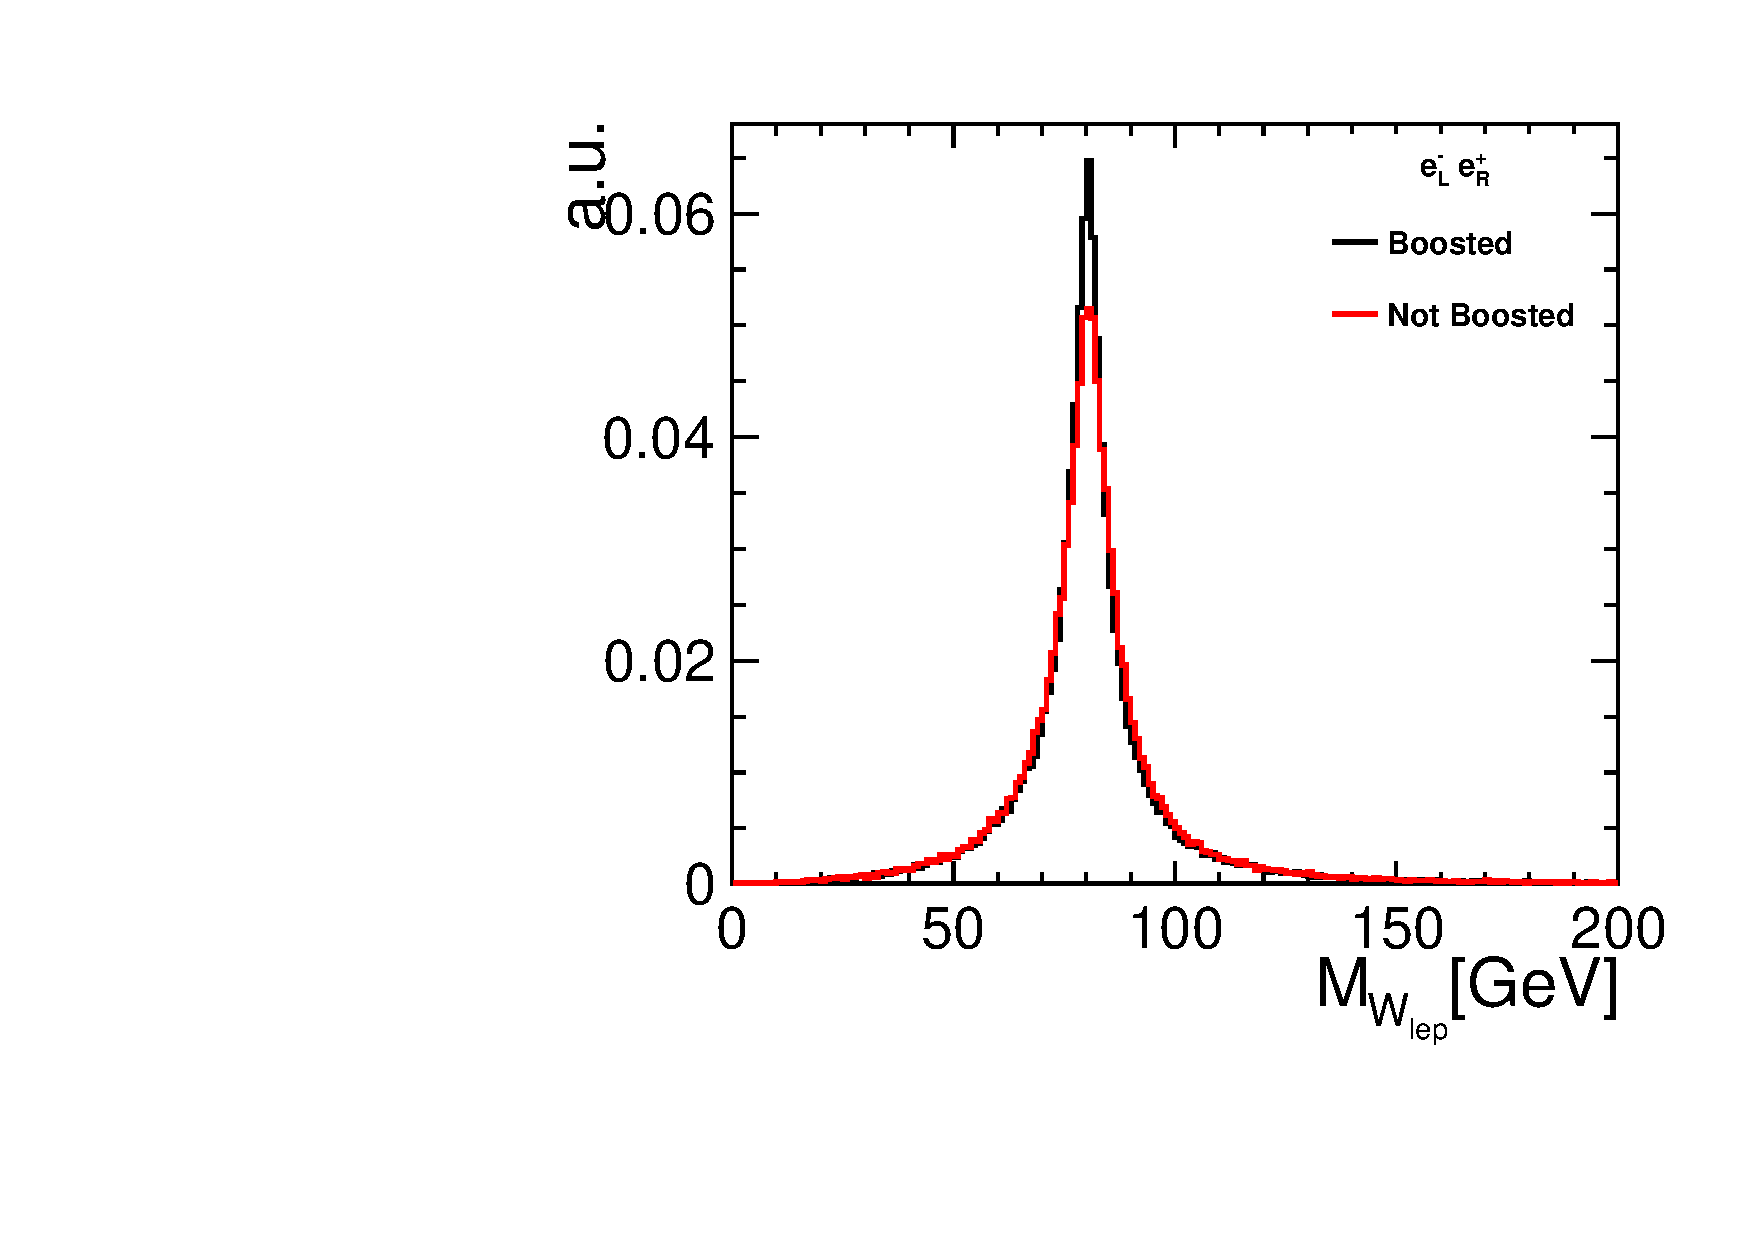
\includegraphics[width=\textwidth]{\imagepath/Boost.pdf}
    \caption{}
    \label{SUBFIG:Boost}
  \end{subfigure}
  \begin{subfigure}[t]{0.45\textwidth}
    \centering
    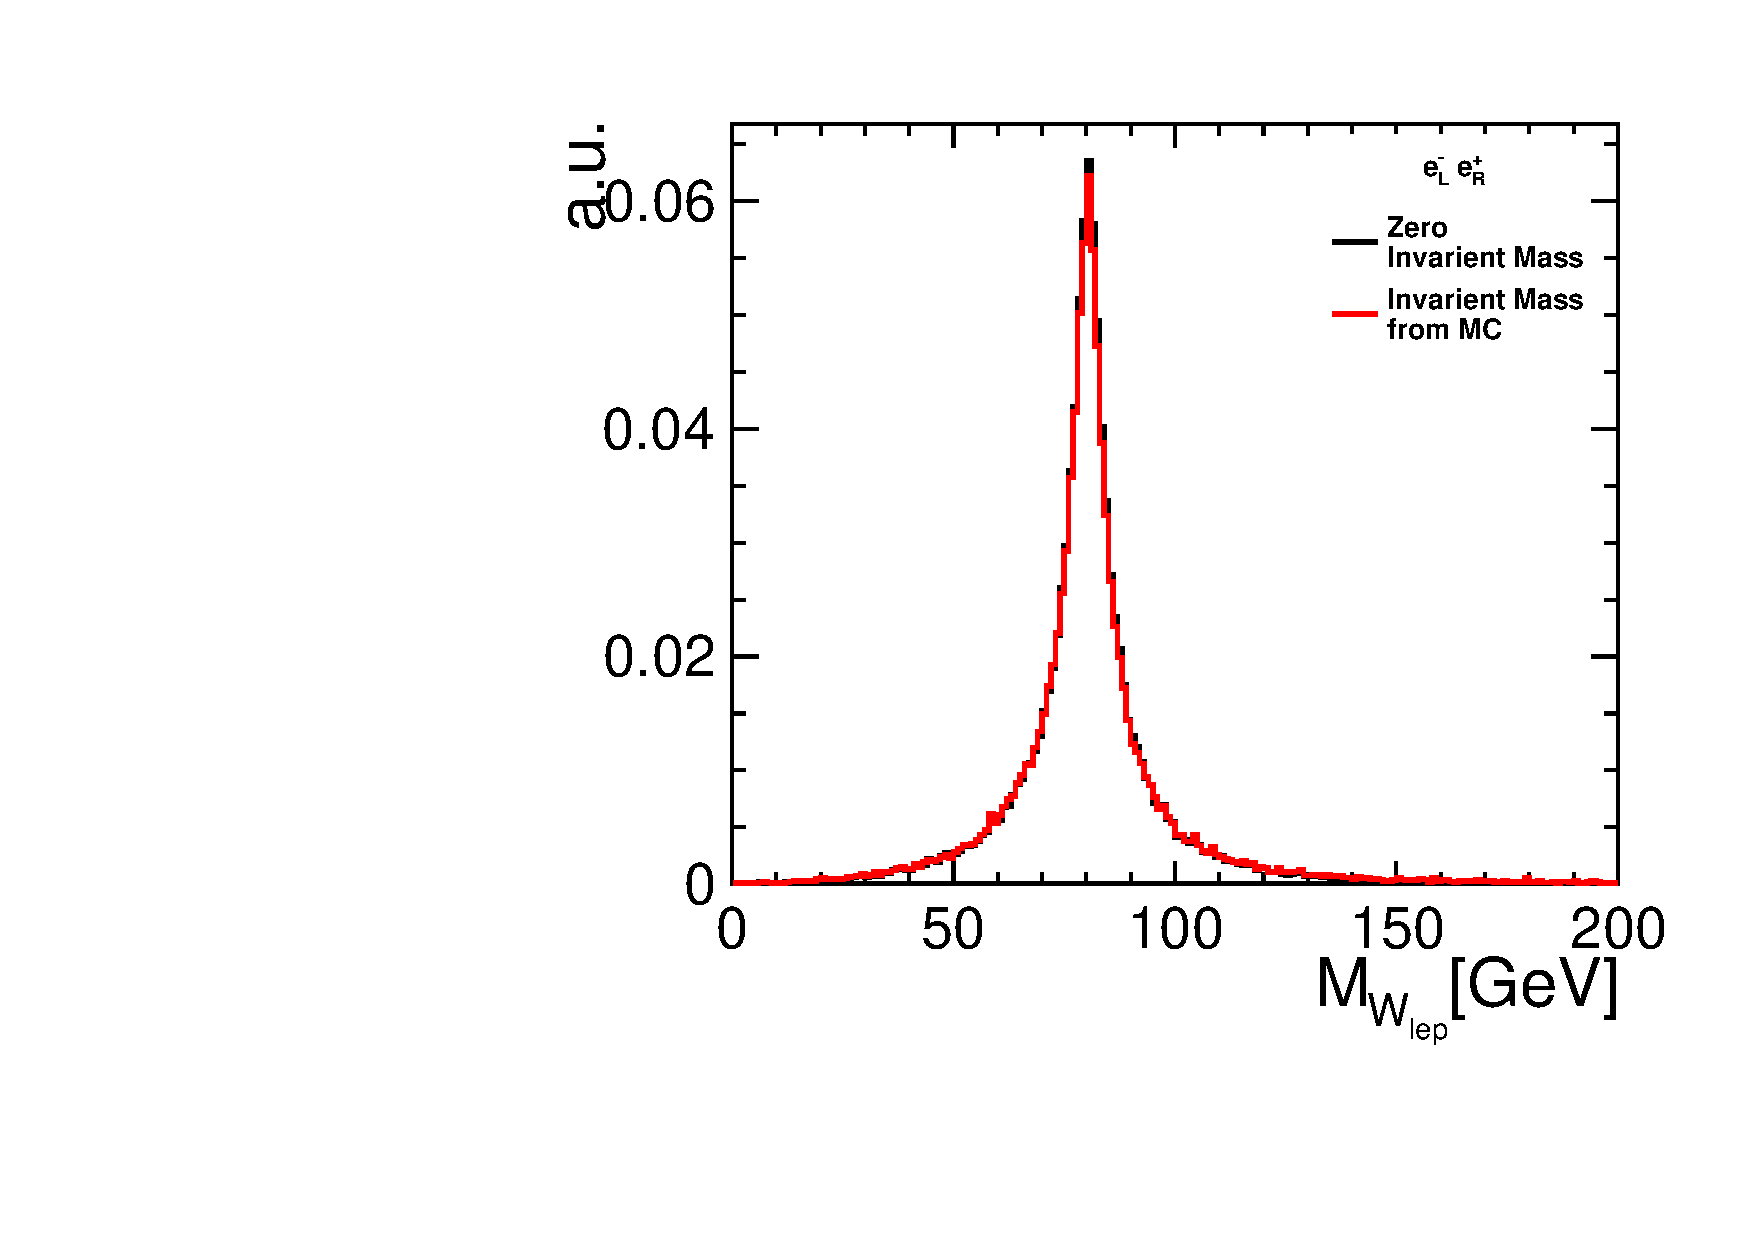
\includegraphics[width=\textwidth]{\imagepath/Mass.pdf}
    \caption{}
    \label{SUBFIG:MassFig}
  \end{subfigure}
  \caption{
    The effect on the reconstructed invariant mass of the leptonically decaying W with different reconstruction methods.
    \subfigref{SUBFIG:MassFig} A Lorentz boost into the center of mass frame is considered.
    \subfigref{SUBFIG:MassFig} A non-zero invariant ISR photon mass, obtained from generator level information, is considered.
    }
  \label{FIG:BoostMass}
\end{figure}

%---------------------------------------------------------------------------------------------------------------------------------------------------------
\subsubsection{ISR invarient mass}
\label{SUBSUBSEC:ISRInvarientMass}
Another assumption that is tested is the non-zero invariant mass of the ISR photon. As two ISR photons are emitted, but only one photon is modelled in the reconstruction, this modelled photon need not satisfy this constraint. The true invariant mass is obtained from the generator level particles and inputed into Equation.~\ref{EQ:Full}, which is derive with this constraint relaxed. Again this is a 'cheat' as this information would not be available in a real detector. This addition had a negligible effect on the reconstructed W mass (see Figure.~\ref{SUBFIG:MassFig}), which could be due to the size of the photon mass indeed being negligible, even if non-zero.

%---------------------------------------------------------------------------------------------------------------------------------------------------------
\subsubsection{Beam Background Removal}
\label{SUBSUBSEC:BeamBackground}
The third check that is performed is the sensitivity of the reconstructed ${m}_{W_{lep}}$  to the beam background. This is done by comparing the two different background removal methods suggested in Section.~\ref{SUBSEC:BeamBackgroundRemoval}. It is found that cheating the beam background removal improved the reconstruction of the two quarks, which can be seen in the reconstruction of the invariant mass of the hadronically decaying W boson (Figure.~\ref{FIG:Cheat}). In particular this cheating greatly suppresses an overestimation tail observed in the properly reconstructed particles. This in turn improves the reconstruction of the visible portion of the system. The ${m}_{W_{lep}}$ on the other hand is generally insensitive to this change. Explaining this is non-trivial due to the fairly complicated nature of the $E_{\gamma}$ formula.
\begin{figure}
    \begin{subfigure}[t]{0.45\textwidth}
      \centering
      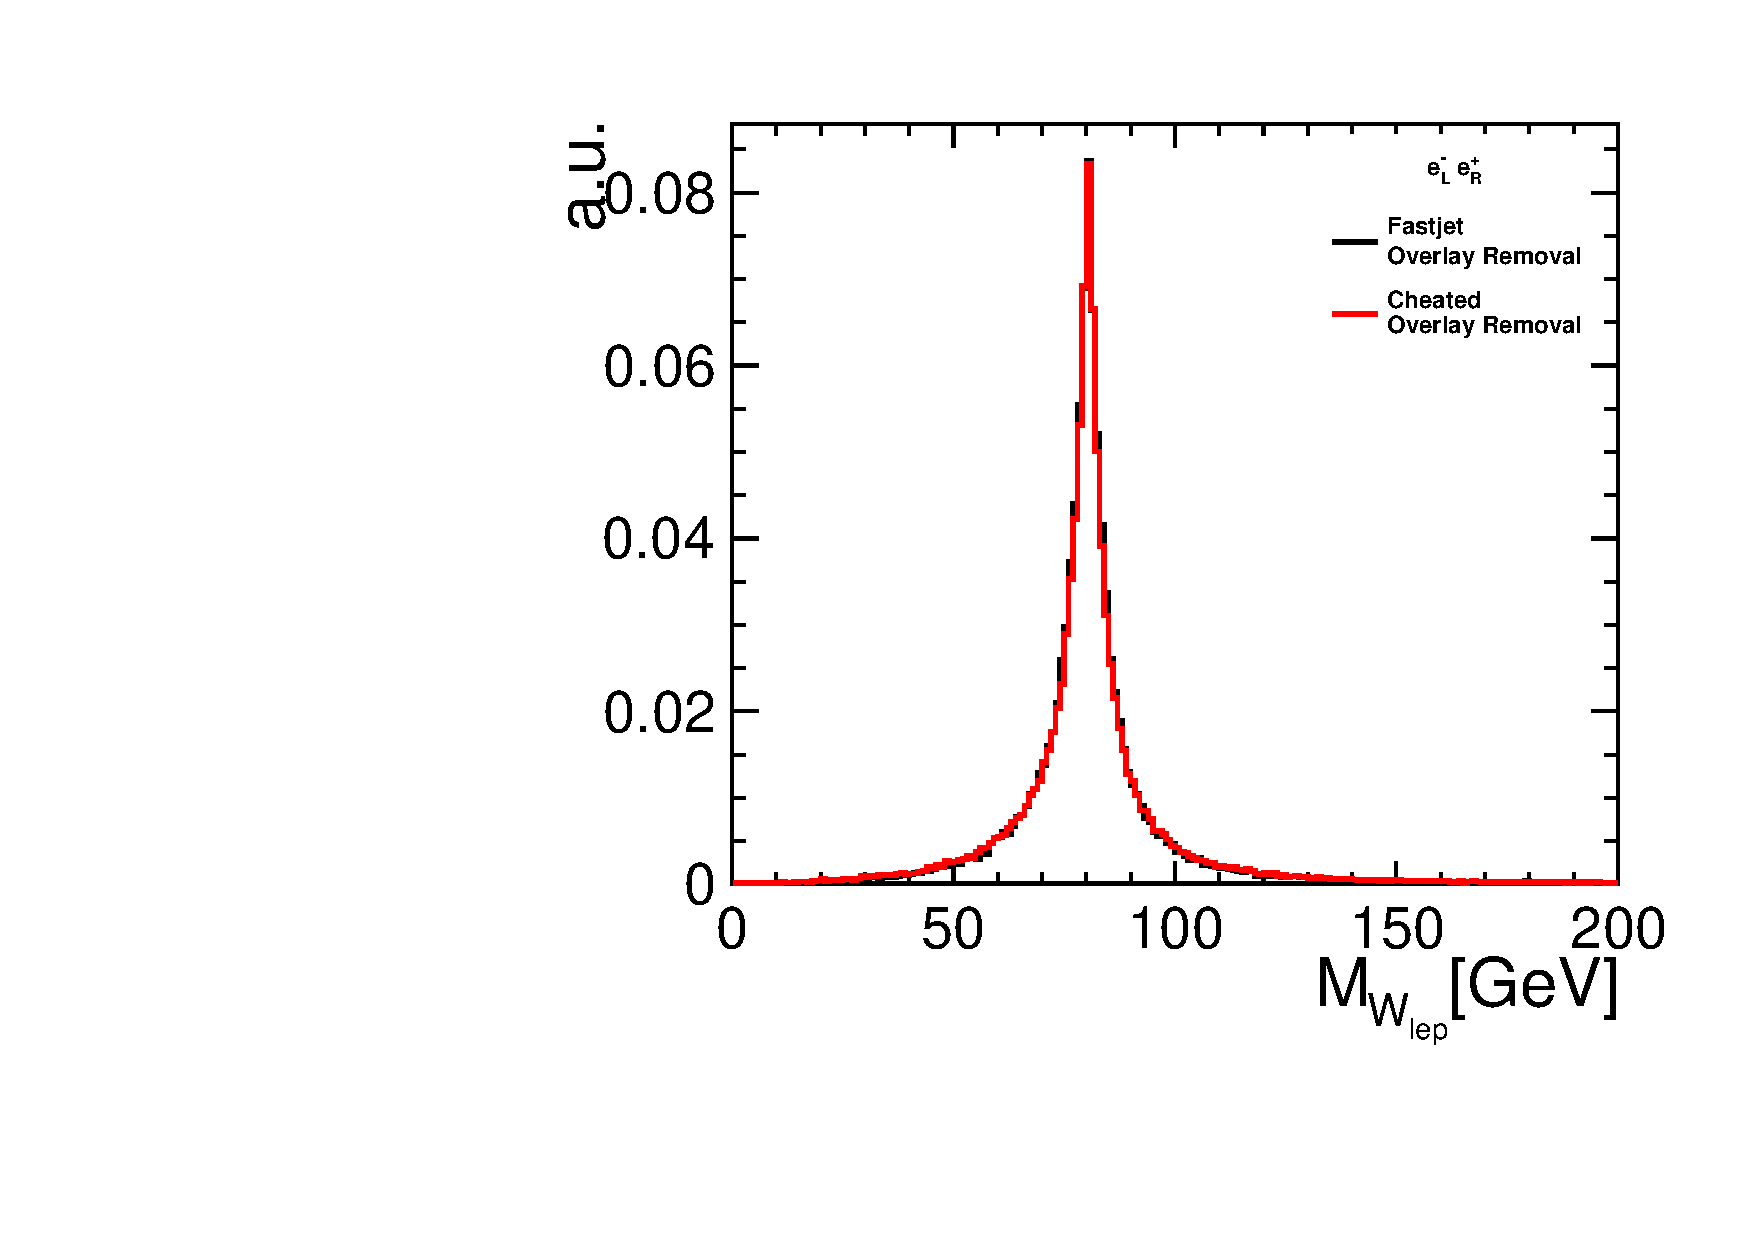
\includegraphics[width=\textwidth]{\imagepath/Lep.pdf}
      \caption{}
      \label{SUBFIG:CheatLep}
    \end{subfigure}
    \begin{subfigure}[t]{0.45\textwidth}
      \centering
      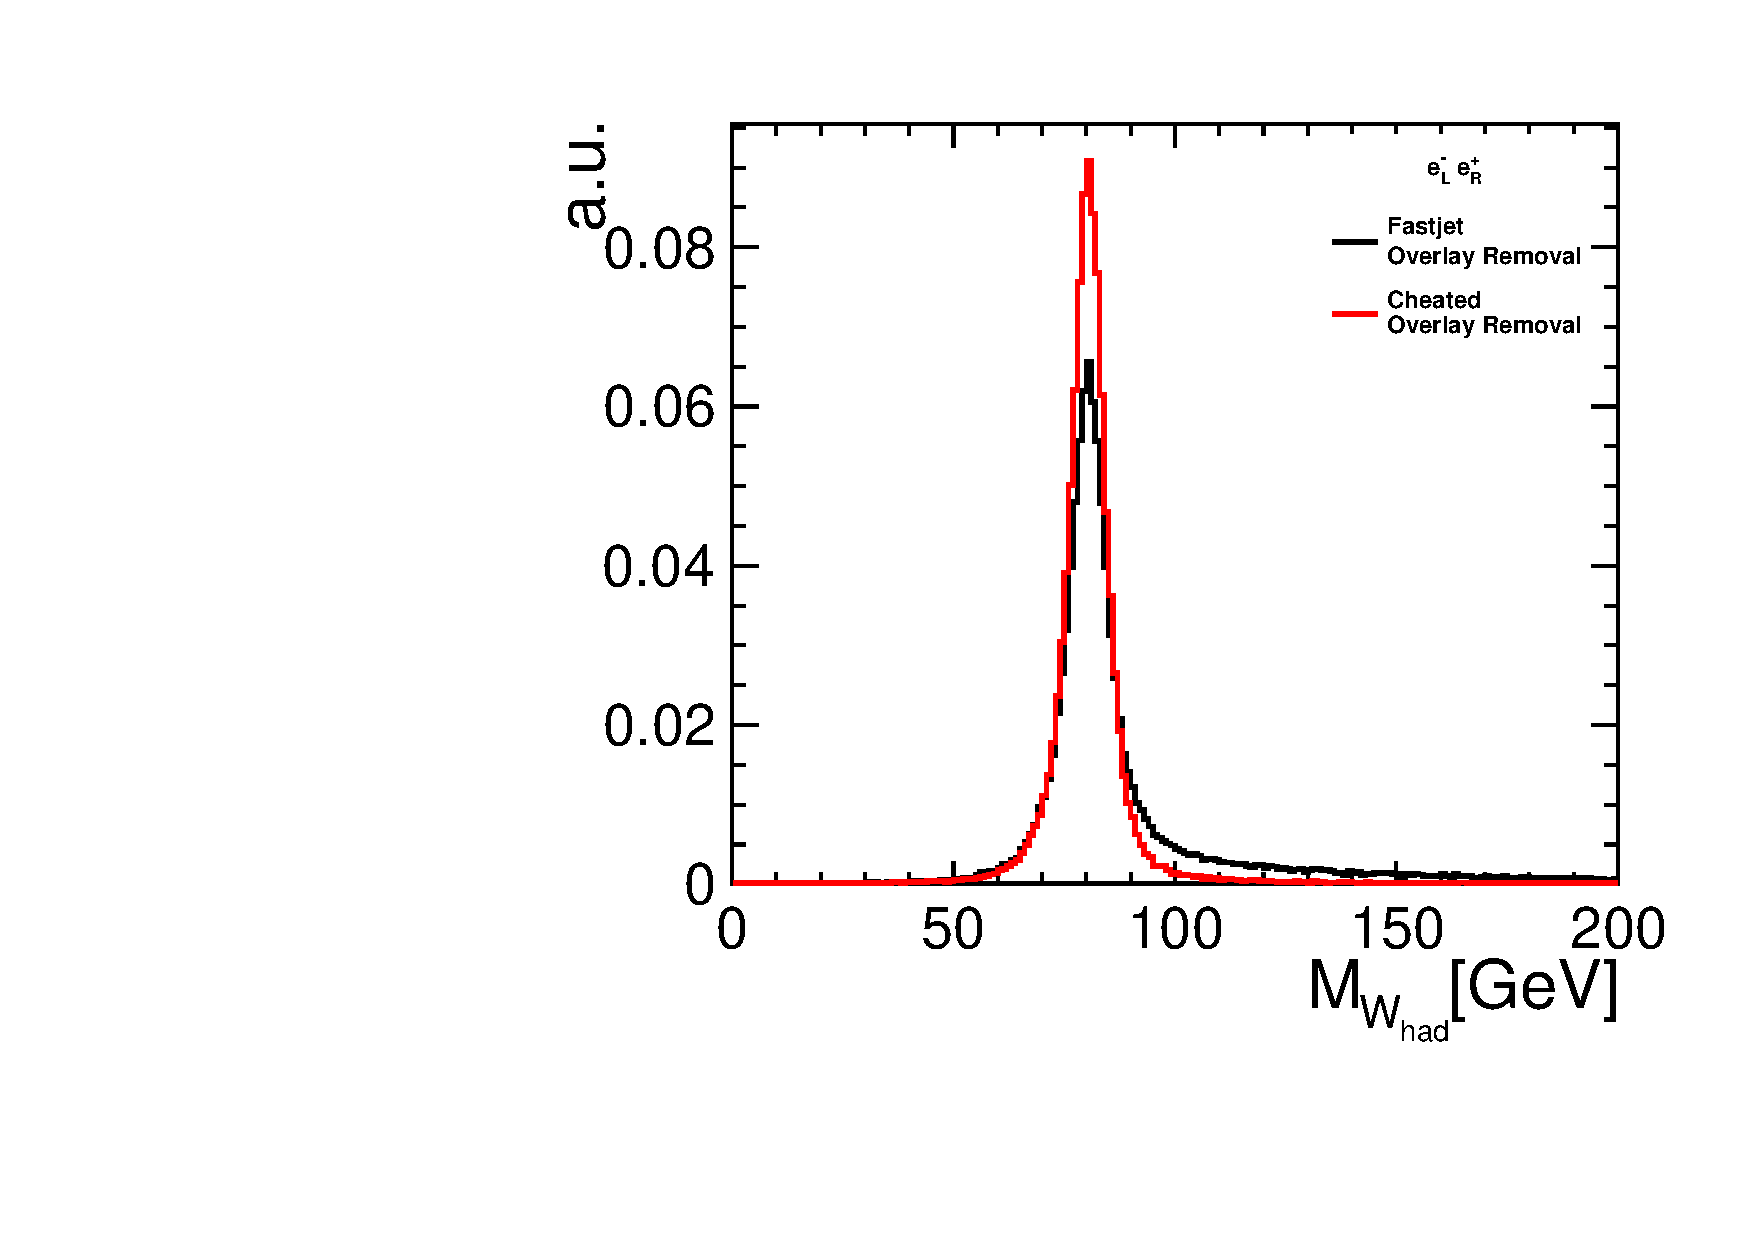
\includegraphics[width=\textwidth]{\imagepath/Jet.pdf}
      \caption{}
      \label{SUBFIG:CheatHad}
    \end{subfigure}
    \caption{
        Plots displaying the effect of cheating the beam background removal on the reconstructed invariant mass of the two W bosons,
        \subfigref{SUBFIG:CheatLep} the leptonically decaying W and \subfigref{SUBFIG:CheatHad} decaying hadronically.
      }
    \label{FIG:Cheat}
\end{figure}

%---------------------------------------------------------------------------------------------------------------------------------------------------------
\subsubsection{Negligible ISR case}
\label{SUBSUBSEC:NoISR}
The ISR energy formula regularly reconstructs a wide range of energies (of order $\pm 20$ GeV) when the true ISR energy is less than 0.5 GeV(see Figure.~\ref{SUBFIG:ZeroPhoton}). Addition of a third solution to the photon energy formula is implemented, where the photon energy, and hence momentum, is set exactly equal to zero. The conservation laws then directly defined the 4-momenta of the neutrino, as it is then the only contribution to the invisible part of the system. As before the estimate of ${m}_{W_{lep}}$ is calculated using all three solutions to $E_{\gamma}$ and the solution that more accurately reconstructed this mass os chosen. Once again this selection may draw more of the background into the peak and introduce a bias. The extent of this is not explored in this report, but it is important to keep into consideration in the following, and any further, analysis. This seems to improve the estimation of ${m}_{W_{lep}}$ as seen in (Figure.~\ref{SUBFIG:Mass3}), although it is unclear if this is a true improvement in the method due this bias.
\begin{figure}
    \begin{subfigure}[t]{0.32\textwidth}
      \centering
      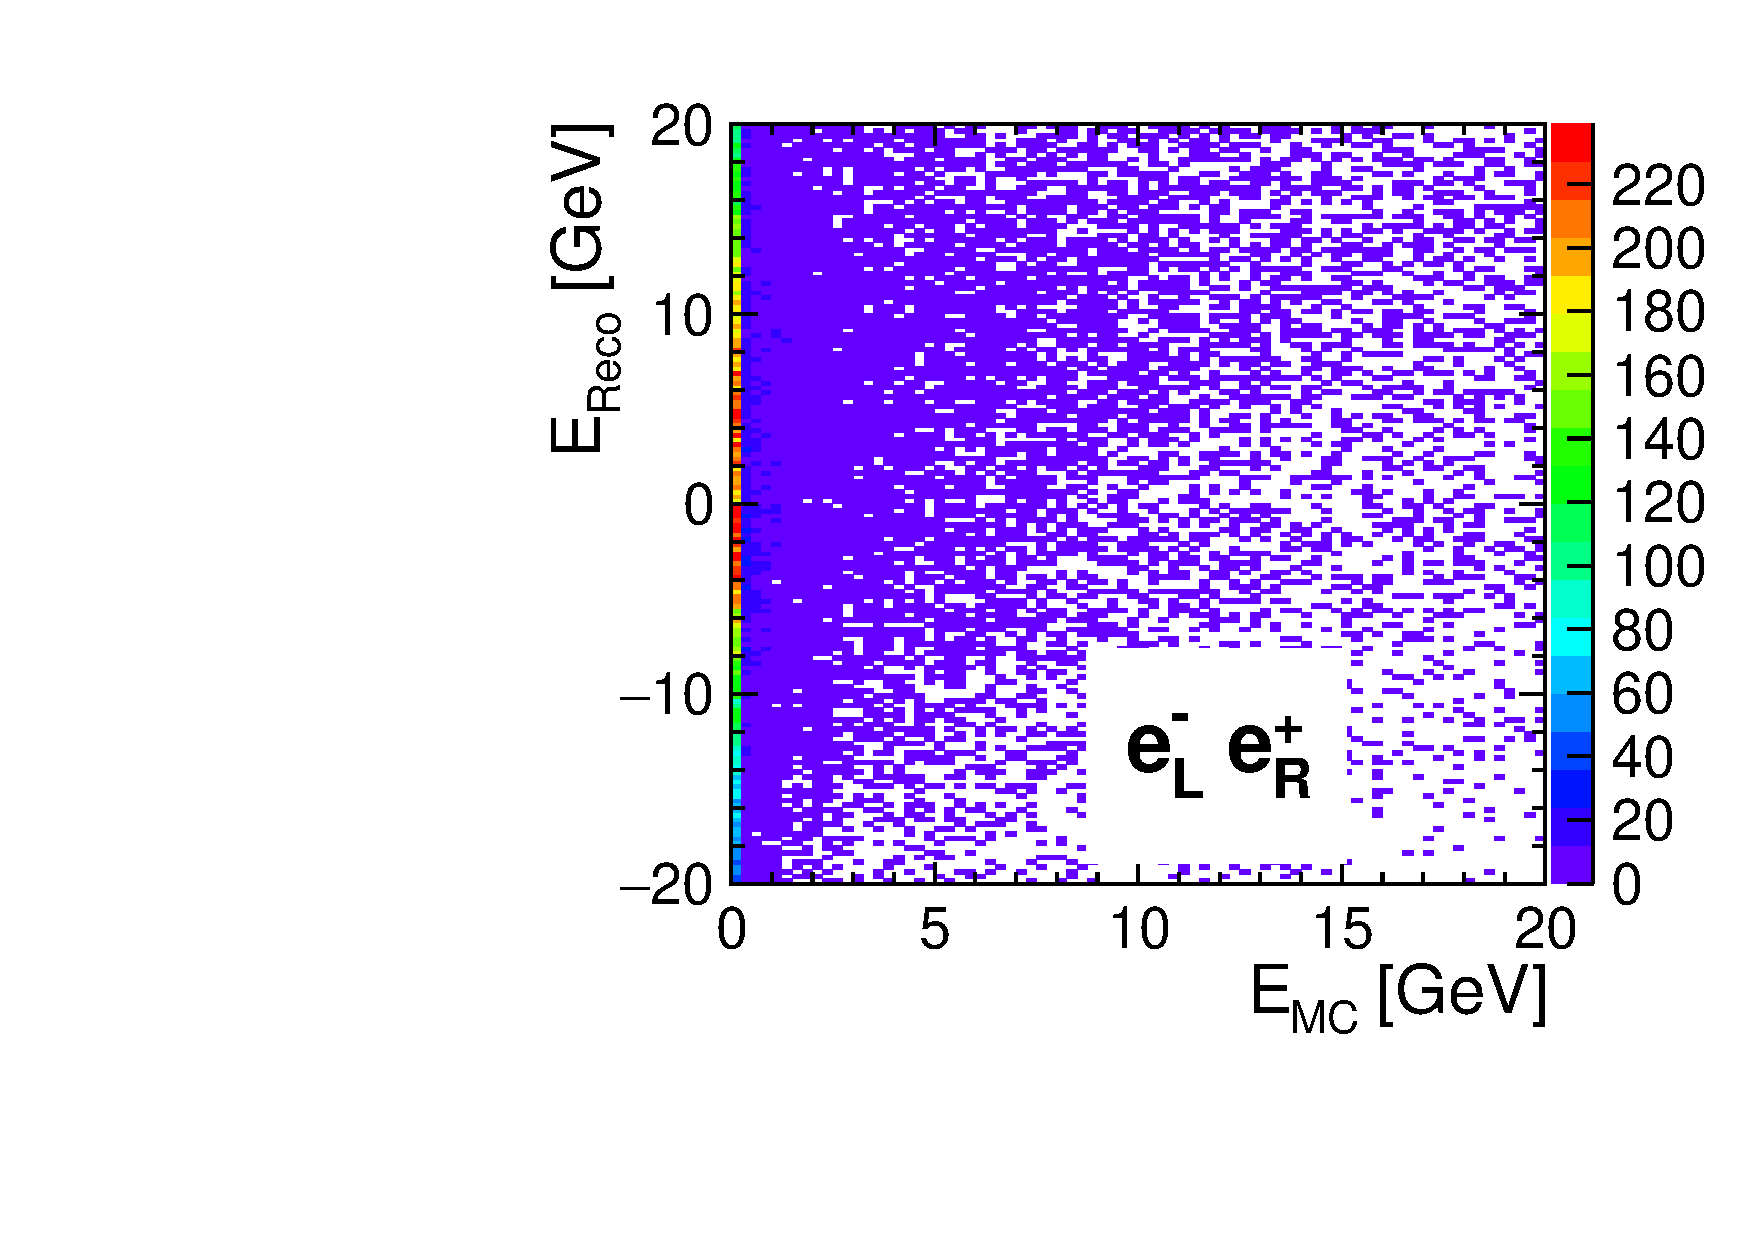
\includegraphics[width=\textwidth]{\imagepath/PhotonEnergy_2D.pdf}
      \caption{}
      \label{SUBFIG:ZeroPhoton}
    \end{subfigure}
    \begin{subfigure}[t]{0.32\textwidth}
      \centering
      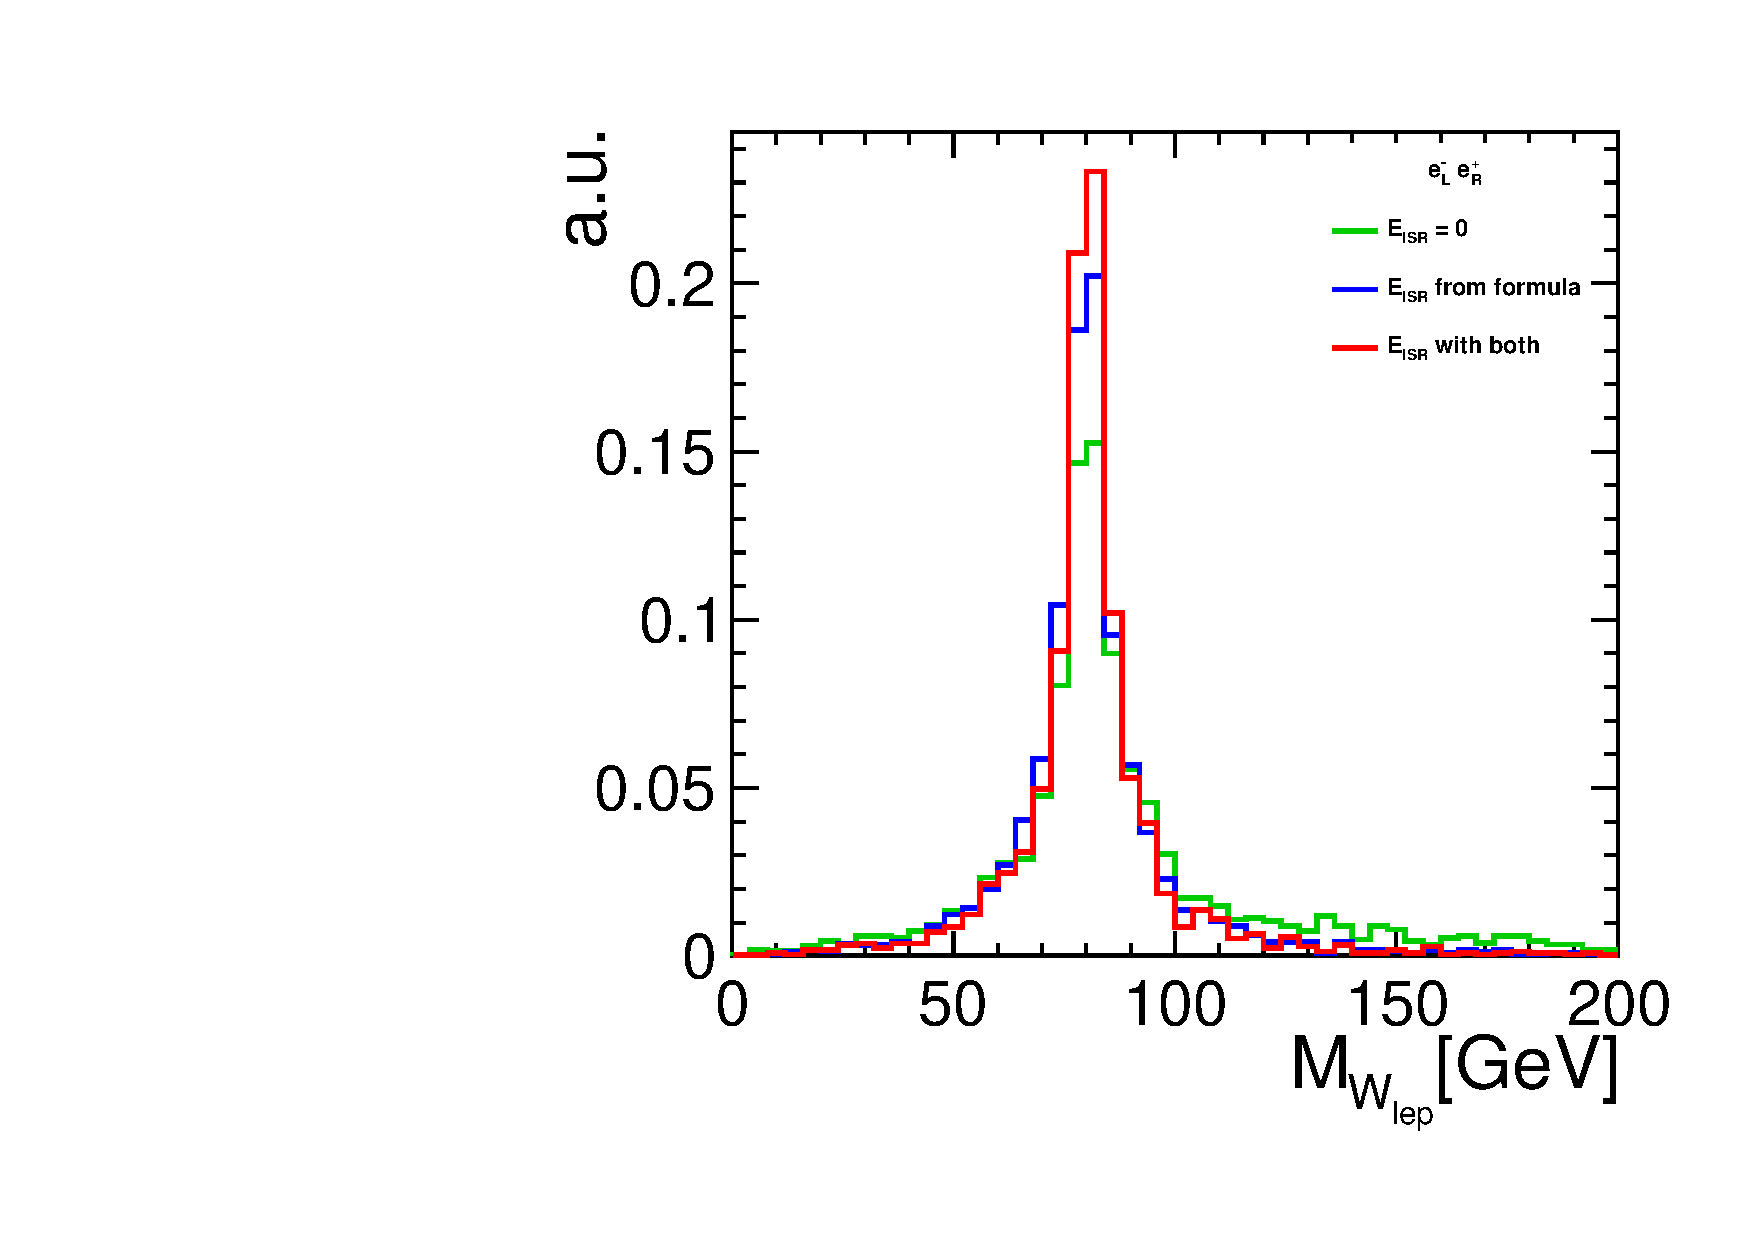
\includegraphics[width=\textwidth]{\imagepath/Mass3.pdf}
      \caption{}
      \label{SUBFIG:Mass3}
    \end{subfigure}
    \begin{subfigure}[t]{0.32\textwidth}
      \centering
      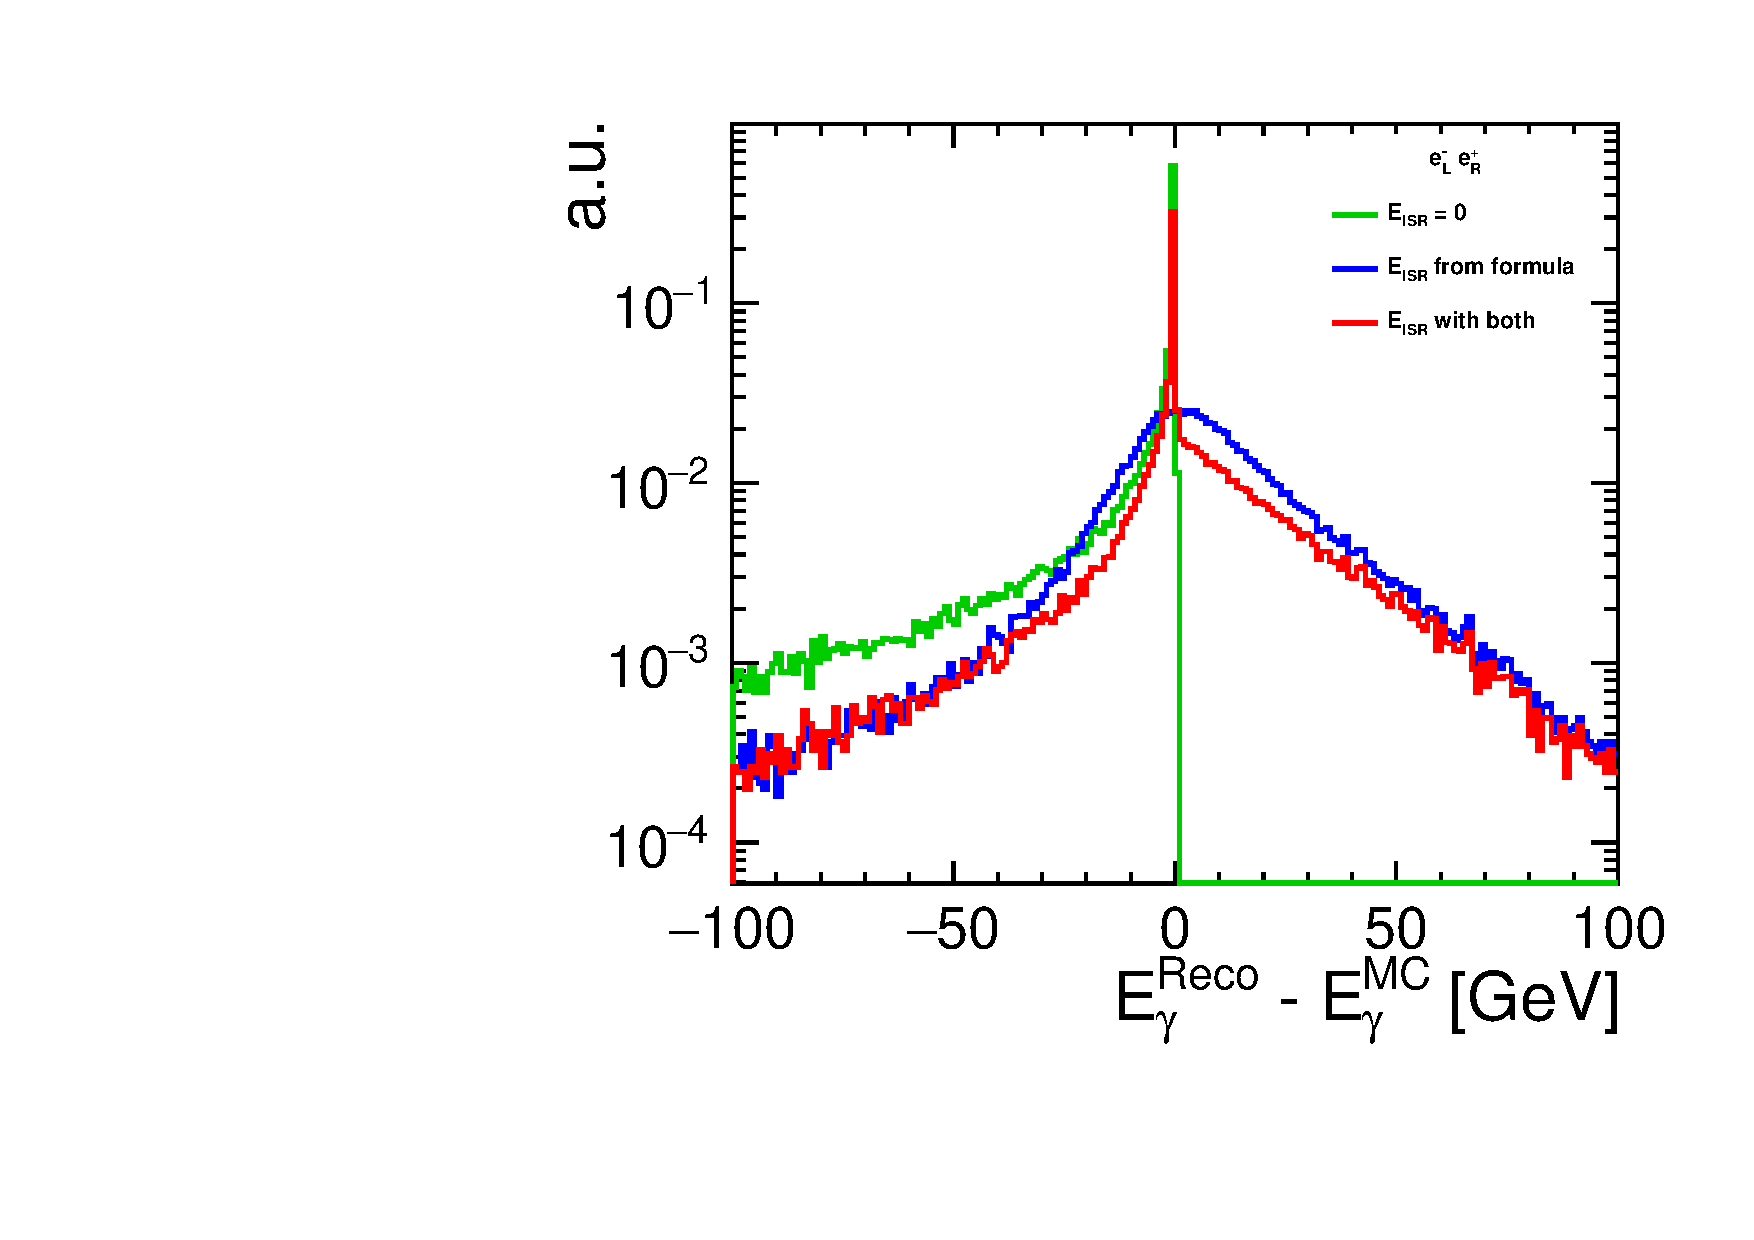
\includegraphics[width=\textwidth]{\imagepath/Photon_Ediff_log3.pdf}
      \caption{}
      \label{SUBFIG:Ediff}
    \end{subfigure}
    \caption{
    \subfigref{SUBFIG:ZeroPhoton} Reconstructed ISR photon energy against the generator level ISR energy.\\
    \subfigref{SUBFIG:Mass3} Reconstruction of the leptonically decaying W mass for the three different ${E}_{\gamma}$ claculation methods .\\
    \subfigref{SUBFIG:Ediff} Log histogram showing the reconstruction of ${E}_{\gamma}$ from the three claculation methods.
     }
    \label{FIG:ZeroPhoton}
\end{figure}
\\\\
As another check of the performance of this edit, a histogram of just $E_{\gamma}^{Reco} - E_{\gamma}^{MC}$ is created (Figure.~\ref{SUBFIG:Ediff}), to see if this improvement in ${m}_{W_{lep}}$ is accompanied by an improvement in the estimation of $E_{\gamma}$. Here it can be seen that the addition of the $E_{\gamma} = 0$ solution  reduces the number of under and over estimates quite significantly. The highest peak at zero , however, claimed by the solution where there is no ISR considered at all (green). This means that sometimes an over/under-estimation of the photon energy returns a better reconstruction of the ${m}_{W_{lep}}$.

%---------------------------------------------------------------------------------------------------------------------------------------------------------%---------------------------------------------------------------------------------------------------------------------------------------------------------
\subsection{Angle extractions}
\label{SUBSEC:AngleExtractions}
From this analysis, complete information about the final state particles, and hence the intermediate W pair, is obtained. From this we can evaluate the angular distributions required for the next section of the analysis. This distributions are extracted from generator level particles, as this is what is being used as input to the Electroweak Polarisation fit.
\\\\
The semileptonic decay of a pair of W bosons is fully described by just 6 angles; the polar coordinates of the ${W}{-}$ in the center of mass frame; the polar coordinated of the lepton in the center of mass frame of the W it decayed from; and the polar coordinated of one of the quarks in the center of mass frame of the boson it decayed from. The $\phi$ coordinate of the ${W}{-}$ is expected to be uniformly distributed and so returns no information about the chiral structure and is not considered in the fit. Further, it is hard to assign a charge to the quarks in their reconstruction, so it is not possible to consistently chose one the the quarks to measure its angles. Hence the quarks polar coordinates are also not considered in this analysis. This leaves just 3 angles as defined in Figure.~\ref{FIG:Angles}, namely the theta coordinate of the ${W}^{-}$ in the centre of mass frame (${\theta}_{{W}^{-}}$), and the theta and phi coordinates of the lepton in the rest frame of the ${W}_{lep}$ it decayed from (${\theta}_{l}^{*}$ and ${\phi}_{l}^{*}$). The polar coordinate system is the same in both frames, with the z axis aligned to the beam-pipe. The same Lorentz boost framework used in Section.~\ref{SUBSUBSEC:CenterOfMassFrame} is implemented here and so this is a computationally very simple task, and the extracted angles are put in the root tree.
\\\\
\begin{figure}
    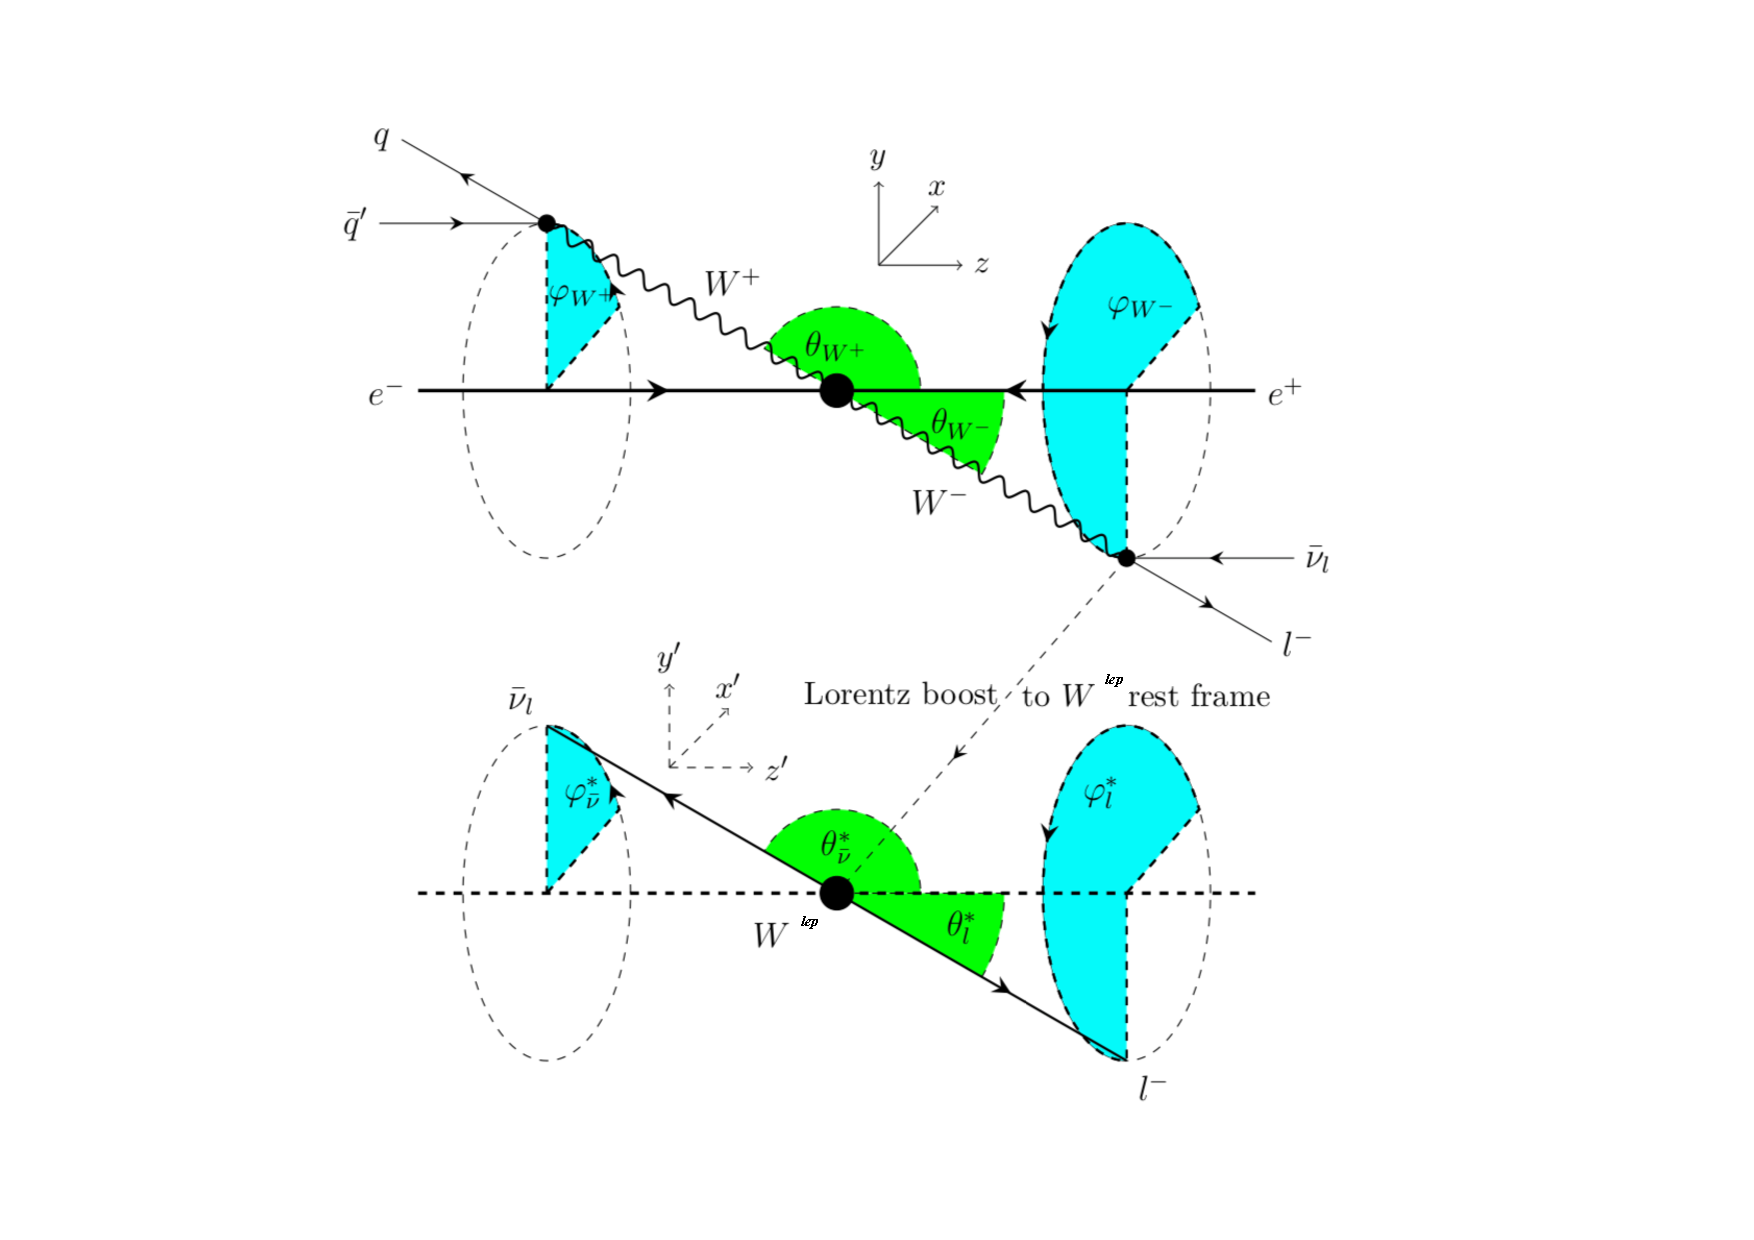
\includegraphics[width=\textwidth]{\imagepath/AngleDiag.pdf}
    \caption{
    Angle definition for the 4-fermion final state from ${W}^{-}$ pair production in the semileptonic channel in which the W− decays leptonically. In the top part, the production angles ${\theta}_{{W}^{-}}$ and ${\theta}_{{W}^{+}}$ are defined by the axis of the initial colliding particles and the direction for the respective boson. The azimuthal angles ${\phi}_{{W}^{-}}$ and ${\phi}_{{W}^{+}}$ describe the rotation around the axis of the initial colliding particles.\\
    The bottom picture shows the angular definition of the decay products of the ${W}^{lep}$ boson in its rest frame. It shows the polar angles ${\theta}_{l}^{*}$ and ${\theta}_{\nubar}^{*}$ and the azimuth angles ${\phi}_{l}^{*}$ and ${\phi}_{\nubar}^{*}$ of the corresponding leptons. The ∗ denotes quantities in the rest frame of the ${W}^{lep}$ boson. (Edited from \cite{Karl:424633})
      }
    \label{FIG:Angles}
\end{figure}

The resulting angular distributions that are obtained are visible in Figure.~\ref{FIG:AngleEfficiencies2}, where the $\theta$ angles have been displayed in terms of their cosine for comparison with previous results \cite{Karl:424633}.
\begin{figure}
    \begin{subfigure}[t]{0.32\textwidth}
        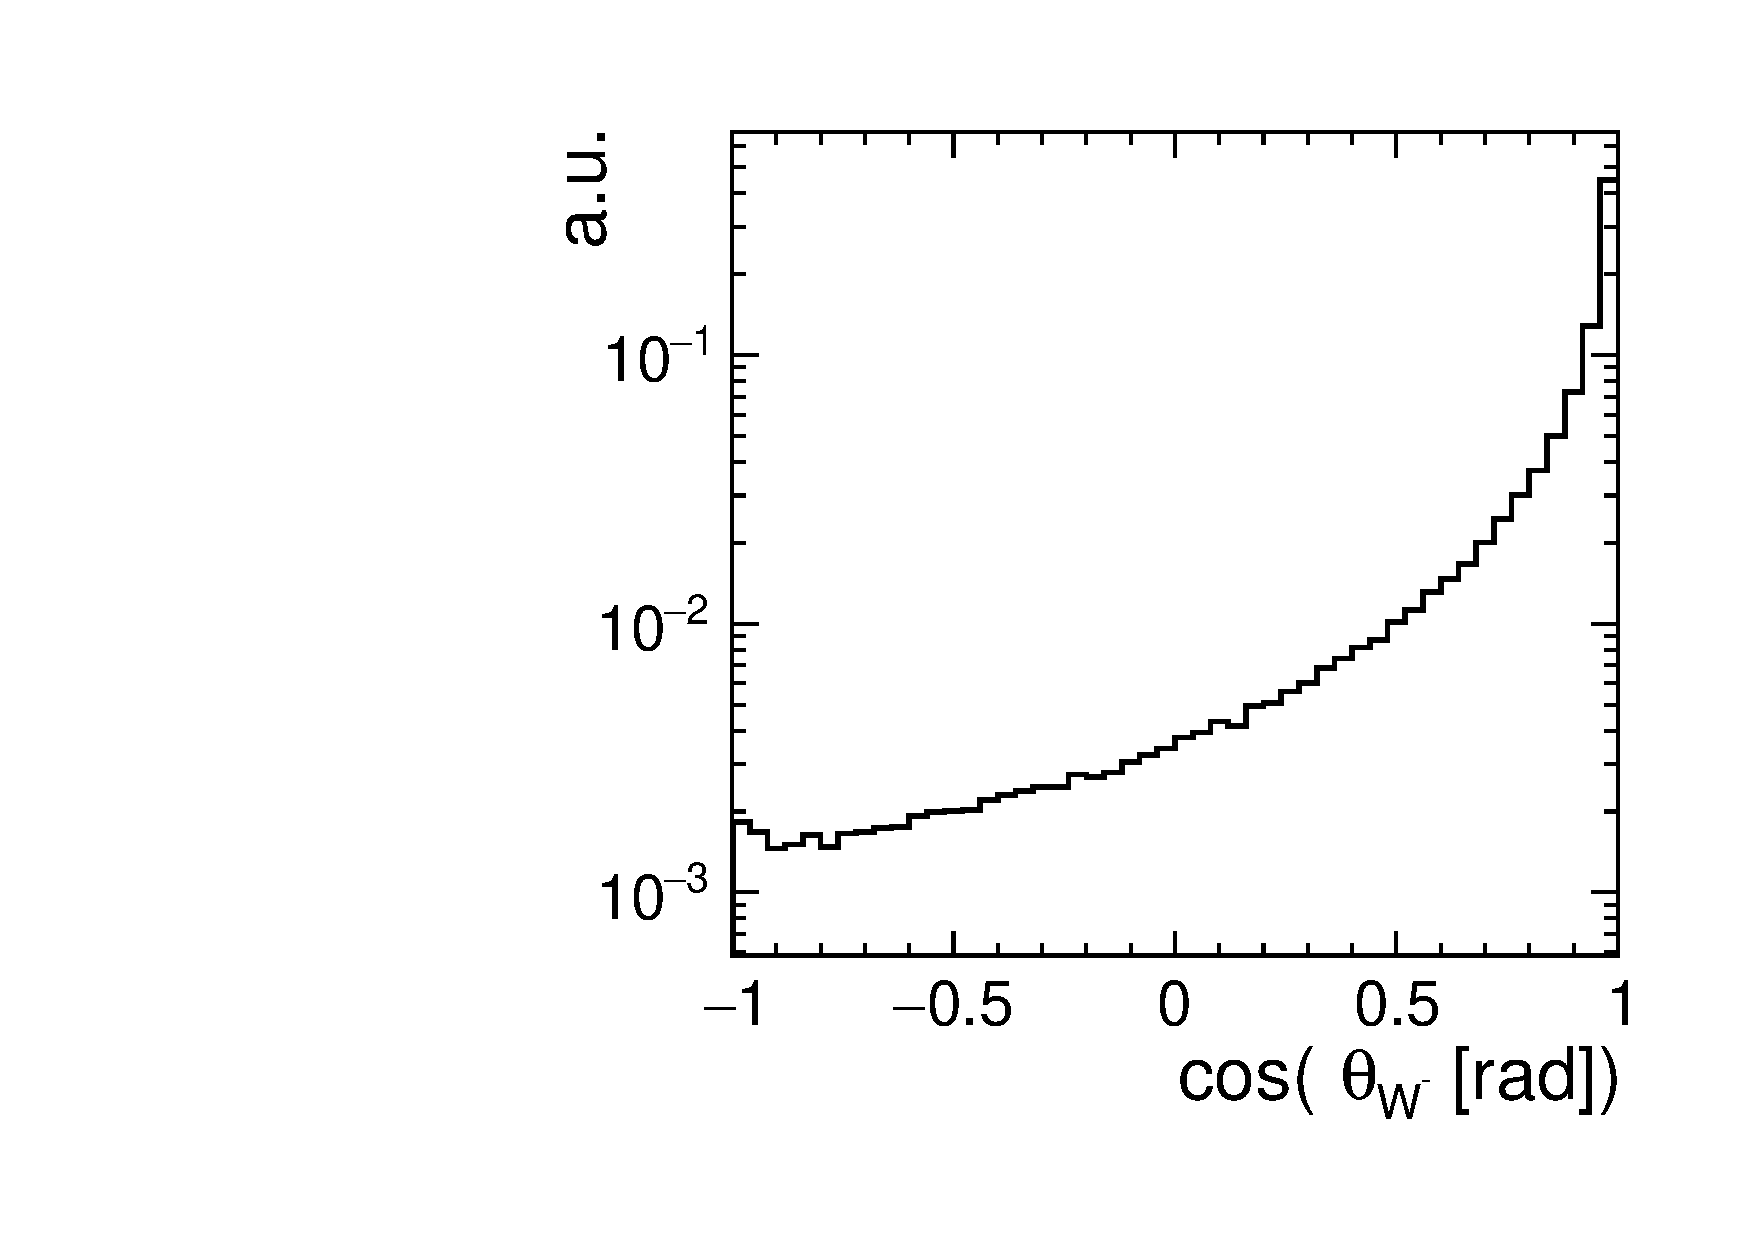
\includegraphics[width=\textwidth]{\imagepath/ThetaMin_cos.pdf}
        \caption{}
        \label{SUBFIG:ThetaMin2}
    \end{subfigure}
    \begin{subfigure}[t]{0.32\textwidth}
        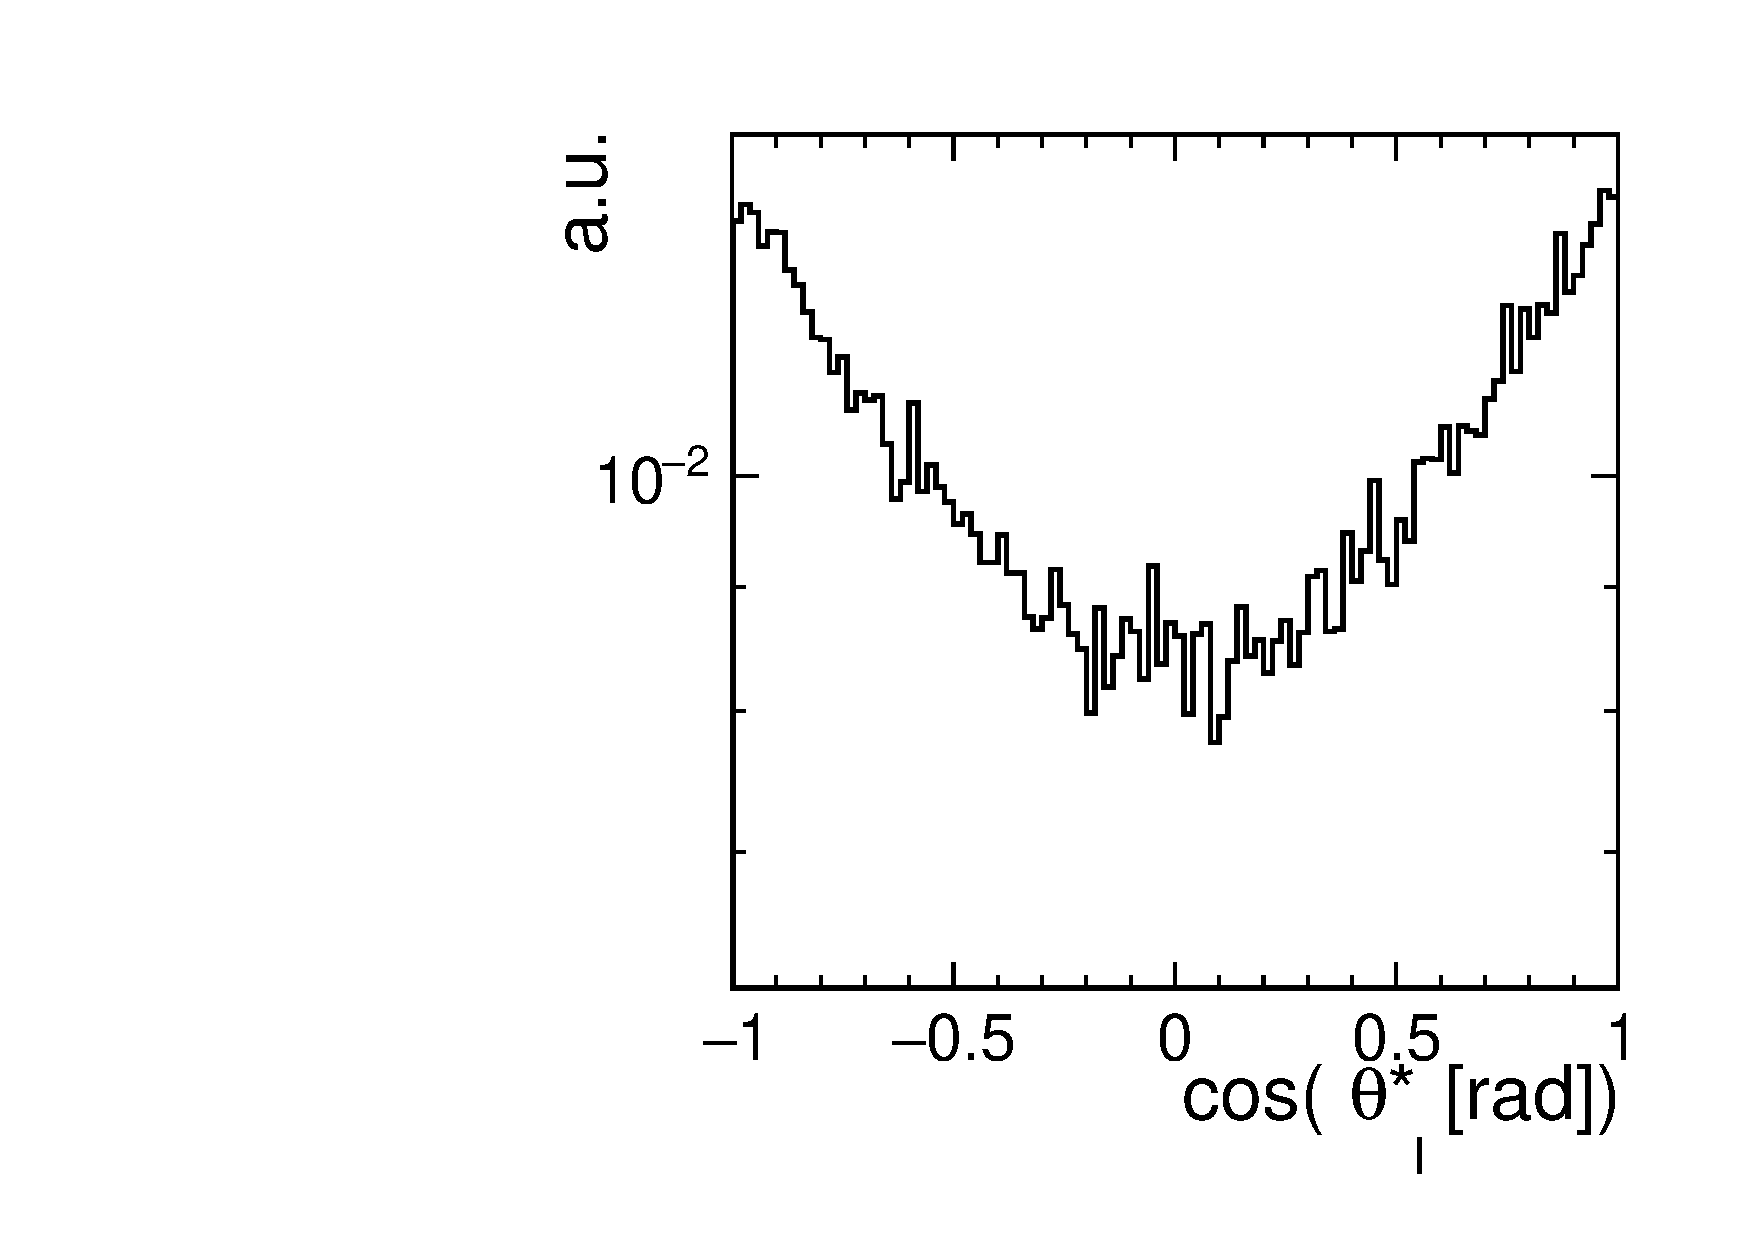
\includegraphics[width=\textwidth]{\imagepath/ThetaLep_cos.pdf}
        \caption{}
        \label{SUBFIG:ThetaLep2}
    \end{subfigure}
    \begin{subfigure}[t]{0.32\textwidth}
        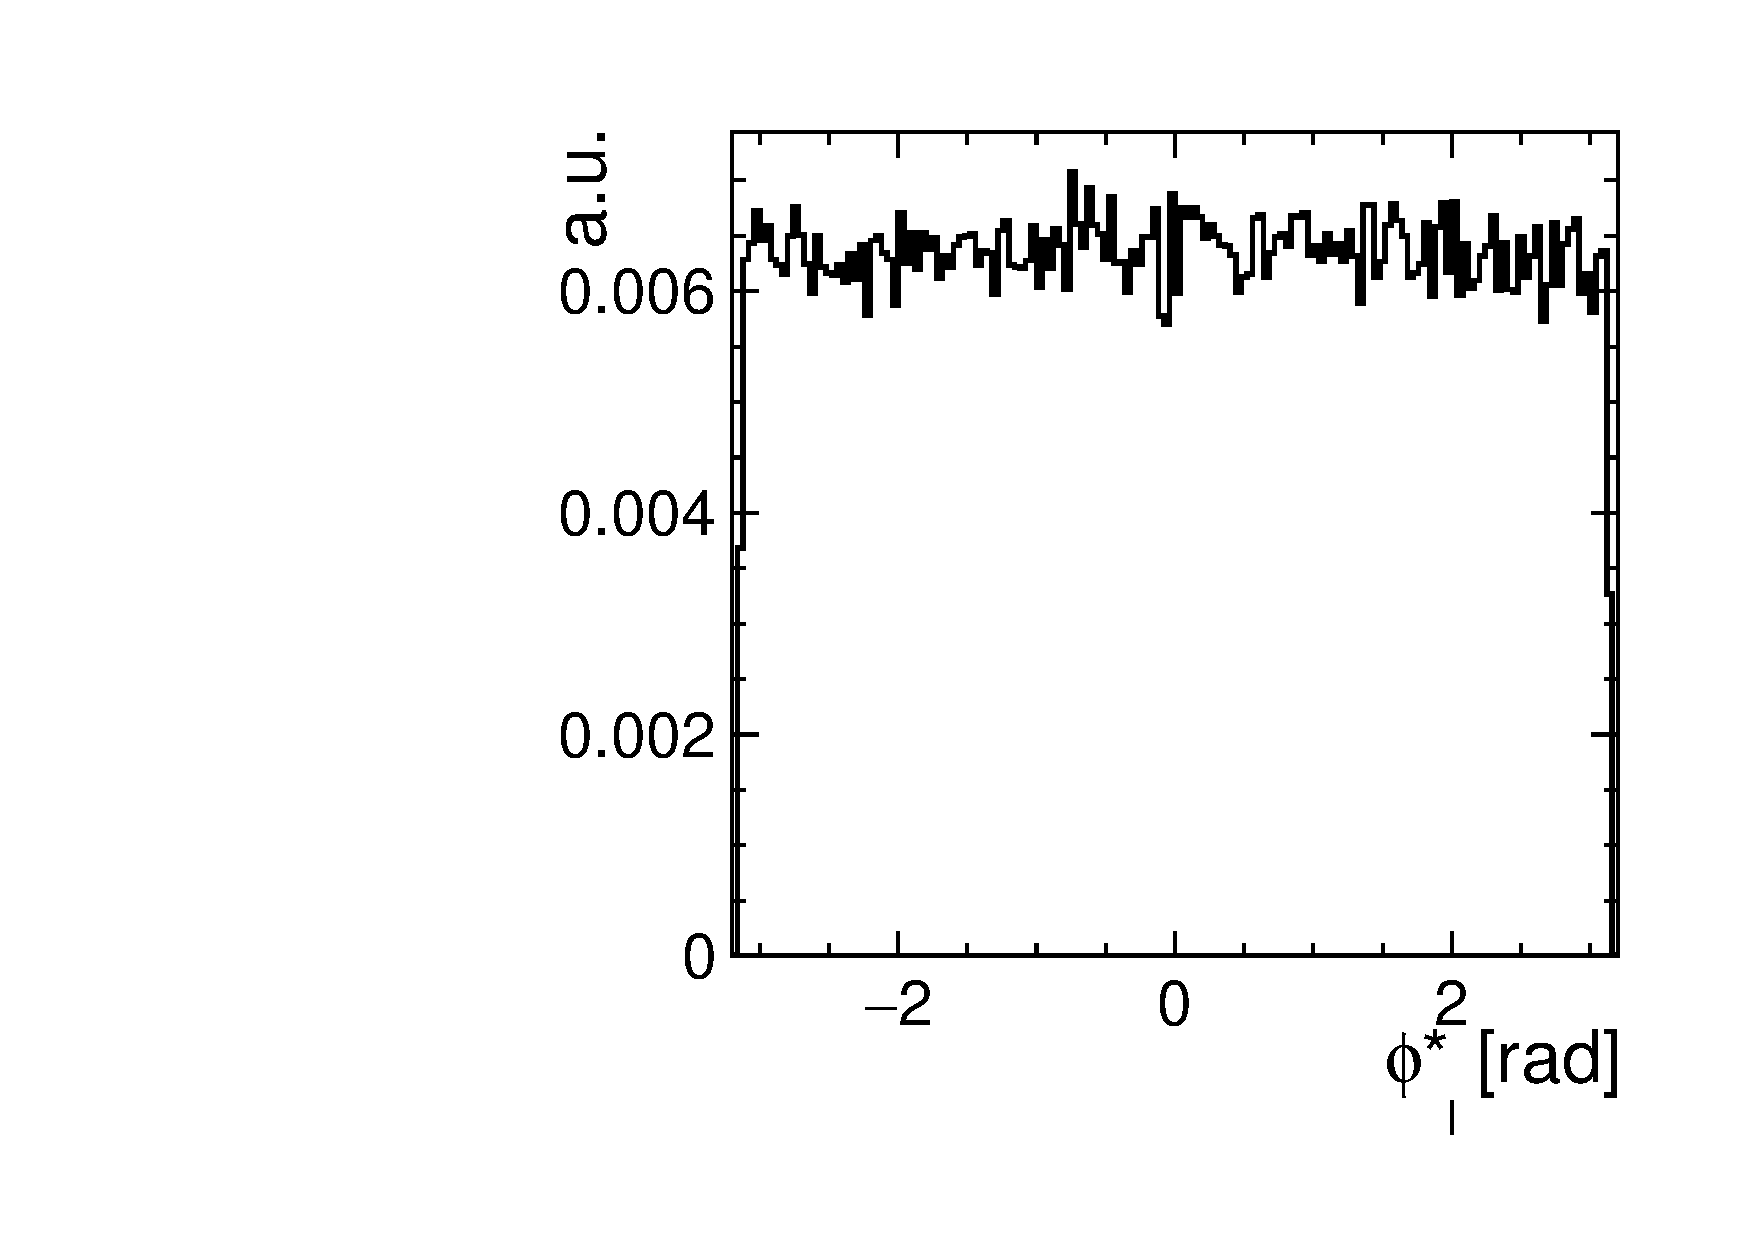
\includegraphics[width=\textwidth]{\imagepath/PhiLep.pdf}
        \caption{}
        \label{SUBFIG:PhiLep2}
    \end{subfigure}\\
    \begin{subfigure}[t]{0.32\textwidth}
        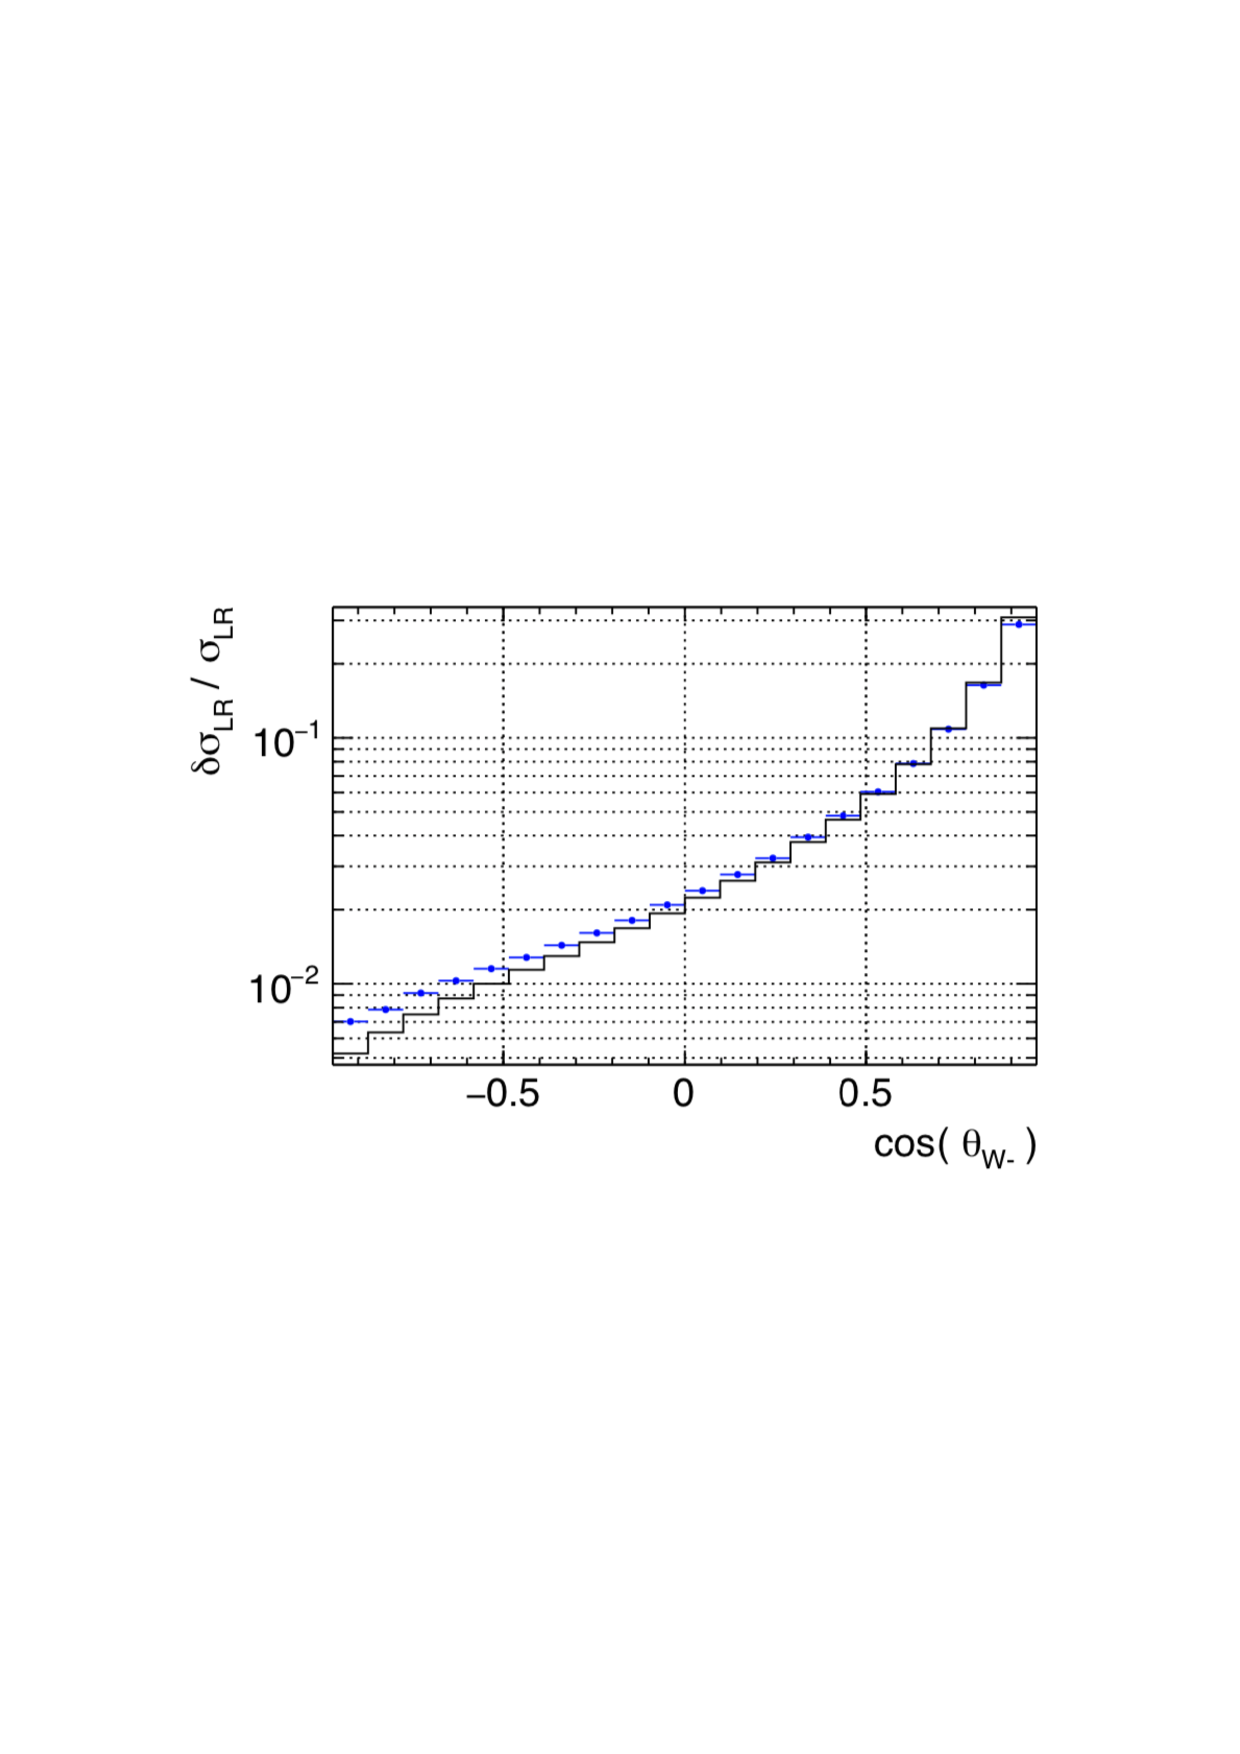
\includegraphics[width=\textwidth]{\imagepath/R_ThetaMin_cos.pdf}
        \caption{}
        \label{SUBFIG:ThetaMinError2}
    \end{subfigure}
    \begin{subfigure}[t]{0.32\textwidth}
        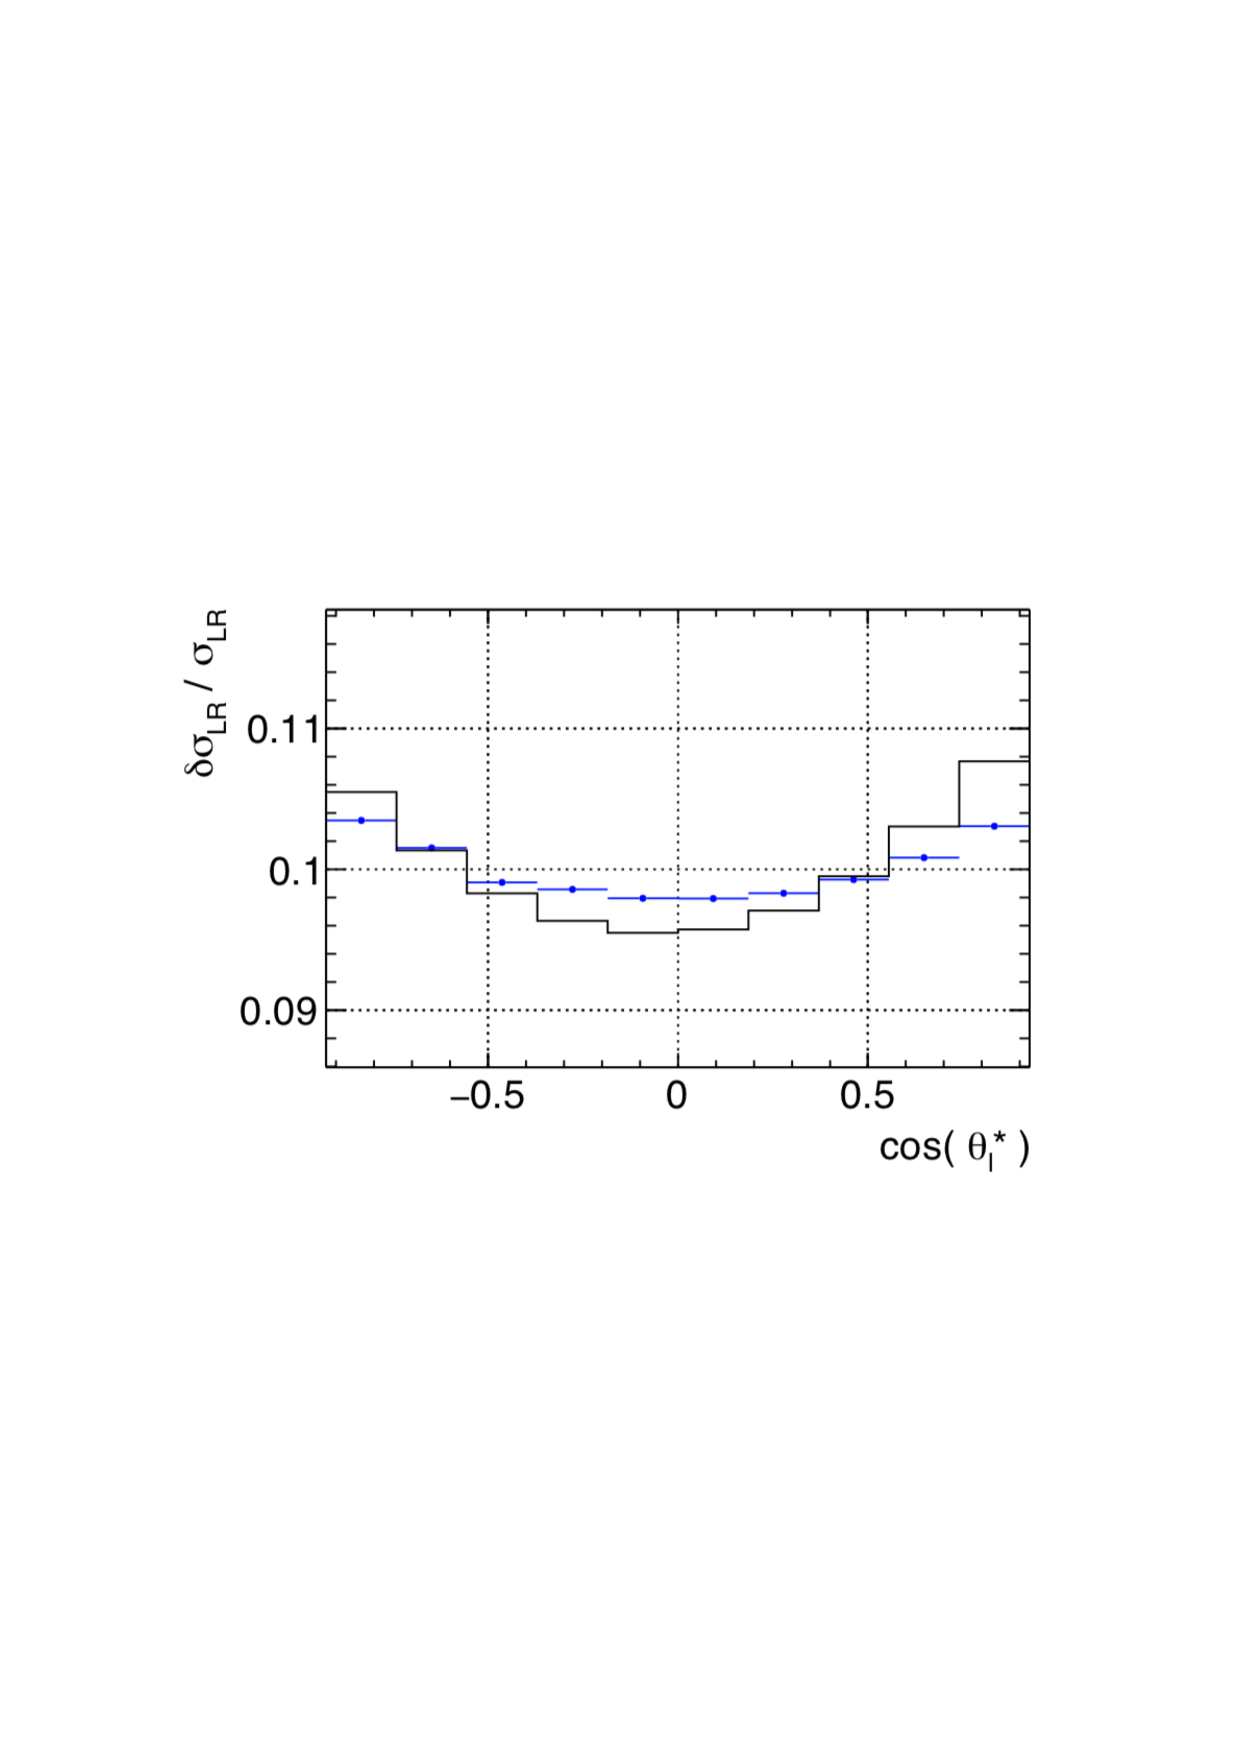
\includegraphics[width=\textwidth]{\imagepath//R_ThetaLep_cos.pdf}
        \caption{}
        \label{SUBFIG:ThetaLepError2}
    \end{subfigure}
    \begin{subfigure}[t]{0.32\textwidth}
        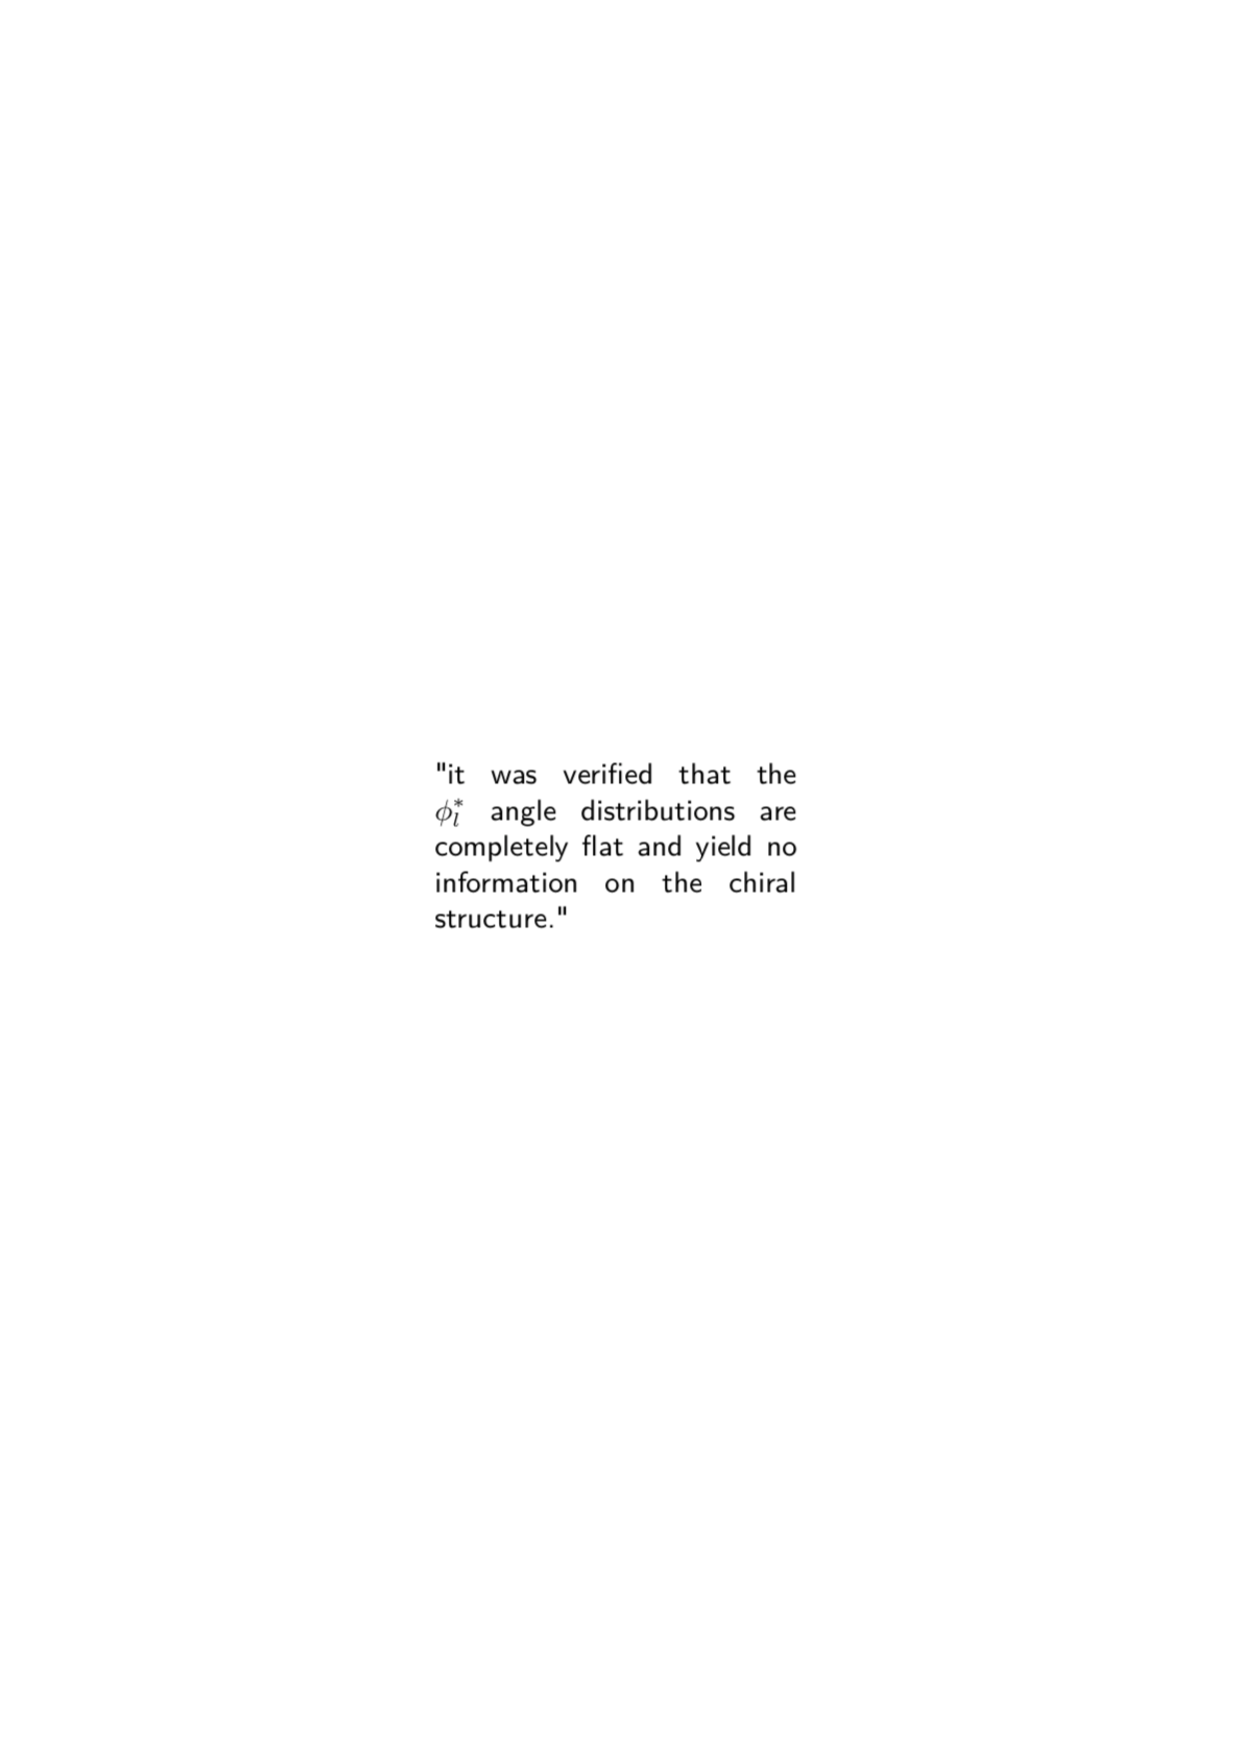
\includegraphics[width=\textwidth]{\imagepath//R_PhiLep.pdf}
        \caption{}
        \label{SUBFIG:PhiLepError2}
    \end{subfigure}
    \caption{
    \subfigref{SUBFIG:ThetaMin2}, \subfigref{SUBFIG:ThetaLep2} and \subfigref{SUBFIG:PhiLep2} are the extracted angles as defined in Figure.~\ref{FIG:Angles}. \\
    \subfigref{SUBFIG:ThetaMinError2}, \subfigref{SUBFIG:ThetaLepError2} are the associated angular distributions currently being input into the Electroweak Polarisation Fit \cite{Karl:424633} and \subfigref{SUBFIG:PhiLepError2} is an extract from the text describing the ${\phi}_{l}^{*}$ distribution
    }
    \label{FIG:AngleEfficiencies2}
\end{figure}
